\documentclass[compress]{beamer}
\mode<presentation>
\setbeamercovered{transparent}
\usetheme{Warsaw}
%\useoutertheme{smoothtree}
\usepackage{multirow}
\usepackage[english]{babel}
\usepackage[latin1]{inputenc}
\usepackage{times}
\usepackage[T1]{fontenc}
\usepackage{xmpmulti}
\usepackage{multicol}
\usepackage{colortbl}

%\setbeamersize{text margin left=.25 in,text margin right=.25 in}
\setbeamersize{text margin left=.15 in,text margin right=.15 in}
\usepackage[authoryear]{natbib}


\usepackage{epstopdf}
\usepackage{xcolor}
\usepackage{latexcolors}
%\usepackage[dvipsnames]{xcolor}
\definecolor{antiquebrass}{rgb}{0.8, 0.58, 0.46}
\definecolor{babyblueeyes}{rgb}{0.63, 0.79, 0.95}
\definecolor{babyblue}{rgb}{0.54, 0.81, 0.94}
\definecolor{bistre}{rgb}{0.24, 0.17, 0.12}
\definecolor{brightlavender}{rgb}{0.75, 0.58, 0.89}
\definecolor{bulgarianrose}{rgb}{0.28, 0.02, 0.03}
\definecolor{slateblue}{rgb}{0.56, 0.74, 0.56}
\definecolor{cordovan}{rgb}{0.54, 0.25, 0.27}
\definecolor{darkbyzantium}{rgb}{0.36, 0.22, 0.33}
%byzantium
\setbeamercolor{structure}{fg=calpolypomonagreen!70, bg= black!60}







\usepackage{tikz}
\usetikzlibrary{shadows,calc}
\usetikzlibrary{shadows.blur}
\usetikzlibrary{shapes.symbols}
\usepackage{hyperref}
\usepackage{booktabs}
\usepackage{colortbl}
\usepackage{multirow}
%%%%%%%%% shaddow image %%%%%
% some parameters for customization
\def\shadowshift{3pt,-3pt}
\def\shadowradius{6pt}
\colorlet{innercolor}{black!60}
\colorlet{outercolor}{gray!05}
% this draws a shadow under a rectangle node
\newcommand\drawshadow[1]{
\begin{pgfonlayer}{shadow}
    \shade[outercolor,inner color=innercolor,outer color=outercolor] ($(#1.south west)+(\shadowshift)+(\shadowradius/2,\shadowradius/2)$) circle (\shadowradius);
    \shade[outercolor,inner color=innercolor,outer color=outercolor] ($(#1.north west)+(\shadowshift)+(\shadowradius/2,-\shadowradius/2)$) circle (\shadowradius);
    \shade[outercolor,inner color=innercolor,outer color=outercolor] ($(#1.south east)+(\shadowshift)+(-\shadowradius/2,\shadowradius/2)$) circle (\shadowradius);
    \shade[outercolor,inner color=innercolor,outer color=outercolor] ($(#1.north east)+(\shadowshift)+(-\shadowradius/2,-\shadowradius/2)$) circle (\shadowradius);
    \shade[top color=innercolor,bottom color=outercolor] ($(#1.south west)+(\shadowshift)+(\shadowradius/2,-\shadowradius/2)$) rectangle ($(#1.south east)+(\shadowshift)+(-\shadowradius/2,\shadowradius/2)$);
    \shade[left color=innercolor,right color=outercolor] ($(#1.south east)+(\shadowshift)+(-\shadowradius/2,\shadowradius/2)$) rectangle ($(#1.north east)+(\shadowshift)+(\shadowradius/2,-\shadowradius/2)$);
    \shade[bottom color=innercolor,top color=outercolor] ($(#1.north west)+(\shadowshift)+(\shadowradius/2,-\shadowradius/2)$) rectangle ($(#1.north east)+(\shadowshift)+(-\shadowradius/2,\shadowradius/2)$);
    \shade[outercolor,right color=innercolor,left color=outercolor] ($(#1.south west)+(\shadowshift)+(-\shadowradius/2,\shadowradius/2)$) rectangle ($(#1.north west)+(\shadowshift)+(\shadowradius/2,-\shadowradius/2)$);
    \shade[outercolor,right color=innercolor,left color=innercolor] ($(#1.north west)+(-\shadowradius/12,\shadowradius/12)$) rectangle ($(#1.south east)+(\shadowradius/12,-\shadowradius/12)$);%Frame
    \filldraw ($(#1.south west)+(\shadowshift)+(\shadowradius/2,\shadowradius/2)$) rectangle ($(#1.north east)+(\shadowshift)-(\shadowradius/2,\shadowradius/2)$);
\end{pgfonlayer}
}
% create a shadow layer, so that we don't need to worry about overdrawing other things
\pgfdeclarelayer{shadow} 
\pgfsetlayers{shadow,main}
% Define image shadow command
\newcommand\shadowimage[2][]{%
\begin{tikzpicture}
\node[anchor=south west,inner sep=0] (image) at (0,0) {\includegraphics[#1]{#2}};
\drawshadow{image}
\end{tikzpicture}}
\usepackage{calligra}

\DeclareMathOperator*{\argmax}{Arg\,max}
\DeclareMathOperator*{\argmin}{Arg\,min}
\newcommand{\norm}[1]{\left\Vert #1 \right\Vert }
\newcommand{\bbetaHat}{ \widehat{\bbeta}}
\newcommand{\bbetaLSE}{ \widehat{\bbeta}_{_{\text{LSE}}}}
\newcommand{\bbetaMLE}{ \widehat{\bbeta}_{_{\text{MLE}}}}
\newcommand{\sqBullet}[1]{  {\tiny \tiny \tiny \qBoxCol{#1!60}{ }} }
%***************
%\newtheorem{thm}{Theorem}
%\documentclass[noinfoline]{imsart}
%\usepackage{amsmath,amstext,amssymb}
%%\usepackage[top=1.5in, bottom=1.5in, left=1.2in, right=1.2in]{geometry}
%% settings
%%\pubyear{2005}
%%\volume{0}
%%\issue{0}
%%\firstpage{1}
%%\lastpage{8}
%\arxiv{arXiv:0000.0000}

%\startlocaldefs
%\numberwithin{equation}{section}
%\theoremstyle{plain}
%\newtheorem{thm}{Theorem}
%\endlocaldefs
\usepackage{lipsum} 
\usepackage{amsmath}
\usepackage{amssymb}
\usepackage{amsbsy} 
\usepackage{amsthm}
\usepackage{mathrsfs}
\usepackage{eufrak}
\usepackage{mathrsfs}
\usepackage{color}
\usepackage{verbatim}
\usepackage{graphicx}
\usepackage{bm}
\usepackage{enumerate}
\usepackage{epstopdf} 
\usepackage{natbib}
\usepackage{undertilde}
%\RequirePackage[colorlinks,citecolor=blue,urlcolor=blue]{hyperref}
%\usepackage{subfig}
\usepackage[final]{pdfpages}

\usepackage{algorithm}  %@subhajit
\usepackage{algpseudocode} %@subhajit
\usepackage{algorithmicx}     %@subhajit
\usepackage{undertilde}


\newcommand{\sphere}{{\mathbb{S}}}
\newcommand{\R}{\mathbb{R}}
\newcommand{\LatentV}{V}
\newcommand{\NC}{m}
\newcommand{\Priorf}{f_{prior}}
\newcommand{\FWOne}[2]{{{}_{1}\Psi _{1}\left[{\begin{matrix}(\frac{#1}{2},\frac{1}{2})\\(1,0)\end{matrix}};#2\right]} 
}


\newcommand{\HyPriorMu}{\thetabf}
\newcommand{\HyPriorAlpha}{\alpha}
\newcommand{\HyPriorBeta}{\beta}
\newcommand{\HyPriorK}{\zeta}
\newcommand{\Indicator}[2]{\mathbb{I}_{_{#1}}({#2 })}
\newcommand{\xb}{\bm{x}}
\newcommand{\bx}{\MakeVec{\bm{x}}}
\newcommand{\bX}{\bm{X}}
\newcommand{\by}{\MakeVec{\bm{y}}}
\newcommand{\bZ}{\bm{Z}}
\newcommand{\bF}{\bm{F}}
\newcommand{\btheta}{\MakeVec{{\bm{\theta}}}}
\newcommand{\Bpi}{\MakeVec{\boldsymbol{\pi}}}
\newcommand{\thetabf}{\MakeVec{\boldsymbol{\theta}}}
\newcommand{\Thetabf}{\boldsymbol{\Theta}}
\newcommand{\taubf}{\MakeVec{\boldsymbol{\tau}}}
\newcommand{\Tr}{Tr}


\newcommand{\bM}{\bm{M}}
\newcommand{\bD}{\MakeVec{\bm{D}}}
\newcommand{\bV}{\MakeVec{\bm{V}}}
\newcommand{\loglikmix}{\mathcal{L}_{\bM,\bD,\bV}}
\newcommand{\hypdc}{{}_0F_1\left(\frac{n}{2},\frac{D_c^2}{4}\right)}


\usepackage{xstring}
\usepackage[normalem]{ulem}
\definecolor{ultramarine}{RGB}{38,29,163}
\newcommand\PalDel[1]{{\color{red} {\sout{#1}}}}
\newcommand\Pal[1]{{\color{ultramarine}{#1}}}
\newcommand\PalRp[2]{\PalDel{#1} \Pal{#2}}
\newcommand\PalCmnt[1]{{\color{ultramarine} {[[[***PAL:  #1 ***]]]}}}

\newcommand{\qedwhite}{\hfill \ensuremath{\Box}}
\newcommand{\SpaceD}{\mathcal{S}_p}
\newcommand{\SpaceM}{\widetilde{\mathcal{V}}_{n,p}}
\newcommand{\SpaceV}{\mathcal{V}_{p,p}}
\newcommand{\SpaceF}{\mathbb{R}^{n,p}}
\newcommand{\StiefelS}{\mathcal{V}_{n,p}}
\newcommand{\SpacePi}{\mathbb{S}_{\pi}}
\newcommand{\ML}{{\cal{ML}}}
\newcommand{\ProdSpace}{\boldsymbol{\Theta}}
\newcommand{\ThetaAndPi}{\Xi}
\newcommand{\ClassML}{\mathcal{C}_{\ML}}


\newcommand{\balpha}{\MakeVec{\bm{\alpha}}}
\newcommand{\bbeta}{\MakeVec{\bm{\beta}}}
\newcommand{\bEta}{\bm{\eta}}
\newcommand{\bd}{{\utilde{\bm{d}}}}
\newcommand{\BoEta}{{\utilde{\boldsymbol{\eta}}}}
%\newtheorem{theorem}{Theorem}[section]
%\newtheorem{theorem}{Theorem}
%\newtheorem{lemma}{Lemma}
%\newtheorem{result}{Result}
\newtheorem{defn}{Definition}
\newcommand{\pdv}[2][]{\frac{\partial#1}{\partial#2}}
\newcommand{\pdvtwo}[2][]{\frac{\partial^2#1}{{\partial#2}^2}}


%\newcommand{\mubf}{\boldsymbol{\mu}}
\newcommand{\mubf}{\MakeVec{\mu}}
\newcommand{\sumI}{ \sum_{i=1}^{n}}
\newcommand{\Ybar}{{\overline{Y}}}

\newcommand{\Expectation}[1]{\mathbb{E}{[#1]}}
\newcommand{\priorXzero}{\Psi}
\newcommand{\iMat}{\mathbf{I}_{p}}

% 
% \newtheorem{thm}{Theorem}[section]
% \newtheorem{cor}[thm]{Corollary}
% \newtheorem{lem}[thm]{Lemma}
%\newtheorem{proposition}{Proposition}

%\newtheorem{theorem}{Theorem}[chapter]%To link the theorem to each chapter uncomment the chapter option
%\newtheorem{lemma}{Lemma}%[theorem]% To link each lemma to a theorem uncomment the theorem option
%\newtheorem{corollary}{Corollary}%[theorem]% To link each corollary to a theorem uncomment the theorem option
% to link a corollary to a chapter change the theorem option to chapter
%\newtheorem{definition}{Definition}%[chapter] %the same is true for both definitions and assumptions
\newtheorem{assumption}{Assumption}%[chapter] %
%\newtheorem{proposition}{Proposition}[chapter]
%\newtheorem{fact}{Fact} %%% added by @subho
\newcommand{\StrongNBD}[2]{S_{#1}{#2}}
\newcommand{\bpi} {\boldsymbol{\pi}}
\newcommand{\bphi} {\boldsymbol{\phi}}
\newcommand{\bb}[1]{\boldsymbol{#1}}
% Definitions of handy macros can go here

\newcommand{\normtwo}[1]{{\left\lVert#1\right\rVert}_2}

\newcommand{\dataset}{{\cal D}}
\newcommand{\fracpartial}[2]{\frac{\partial #1}{\partial  #2}}
\newcommand{\Lesbegue}[1]{\mu_{\btheta_{#1},\bpi_{#1}}}
\newcommand{\fthetapi}[1]{f_{\btheta_{#1},\bpi_{#1}}}
% Heading arguments are {volume}{year}{pages}{submitted}{published}{author-full-names}
\newcommand{\doublehat}[1]{%
    \settoheight{\dhatheight}{\ensuremath{\widehat{#1}}}%
    \addtolength{\dhatheight}{-0.35ex}%
    \widehat{\vphantom{\rule{2pt}{\dhatheight}}%
    \smash{\hspace{-0.5mm}\widehat{#1}}}}

\newcommand{\hyp}{{}_0F_1\left(\frac{n}{2},\frac{D^2}{4}\right)}
\newcommand{\hypinline}{{}_0F_1\left({n}/{2},{D^2}/{4}\right)}

\newcommand{\partialhyp}[1]{\frac{\partial}{\partial\,{d_{#1}}}\,\left[\hyp\right]}

\newcommand{\fracProbZ}[1]{\frac{\langle Z_{ic} \rangle \, #1}{\sum_{i=1}^{N} \langle Z_{ic}\rangle  } }
\newcommand{\EmVar}[1]{\widetilde{#1}^{(c)}}

\newcommand{\IMDY}{{\it{CCPD}}}
\newcommand{\JMDY}{{\it{JCPD}}}

\newcommand{\DYlang}{\frac{\exp(\nu\,\bEta^T\bd)}{{\left[{}_0F_1\left(\frac{n}{2},\frac{D^2}{4}\right)\right]}^{\nu}}}

\newcommand{\logDYlang}{\nu\,\bEta^T\bd - \nu\,\log\left({}_0F_1\left(\frac{n}{2},\frac{D^2}{4}\right)\right)}

\newcommand{\lhyp}{\log\left({}_0F_1\left(\frac{n}{2},\frac{D^2}{4}\right)\right)}

%\jmlrheading{1}{2000}{1-48}{4/00}{10/00}{SS \& JH \& AB}

% Short headings should be running head and authors last names

%\ShortHeadings{BDP and cIBP}{SS \& JH \& AB}
%\firstpageno{1}

\newcommand{\diam}[1]{{{#1}^{\ast}}}

%%% coloring option %%%
\definecolor{auburn}{rgb}{0.53, 0.1, 0.5}
\newcommand{\sss}{\color{auburn}}  %%% for Subhajit
\newcommand{\sse}{\color{black}}
\newcommand{\attn}{\color{red}}
\newcommand{\rms}{\color{magenta}}  %%% for Riten
\newcommand{\rme}{\color{black}}
\newcommand{\MLDensity}{f_{\ML}}
\setlength{\parindent}{0cm}
\newcommand{\posterior}

\newcommand{\variableX}{\bd}
\newcommand{\funch}{\mathfrak{h}}
\newcommand{\IndVzero}[1]{\mathbb{I}({X\in \mathcal{V}^{#1}_0})}
\newcommand{\Rnp}{\mathbb{R}^{n \times p}}
\newcommand{\Rpp}{\mathbb{R}^{p \times p}}
\newcommand{\vecnorm}[1]{\lVert #1\rVert}

\newcommand{\etapsiD}{\eta_{\priorXzero}}
\newcommand{\BoEtapsiD}{\BoEta_{\priorXzero}}

\newcommand{\DMp}{\mathcal{D}^{p \times p}}
\newcommand{\Rplus}{\mathbb{R}_{+}}
\newcommand{\prodMeasure}{\Upsilon}

\newcommand{\m}{{\bf m_{\BoEta}}} 
\newcommand{\SetWithMode}{\mathcal{S}}
\newcommand{\SetWithModePrime}{\mathcal{S}}
\newcommand{\TargetComp}{\mathcal{S}^{\star}}

\newcommand{\ConstCondDen}{K_{\nu, \BoEta}} 

\newcommand{\hyparam}[2]{
    \IfEqCase{#1}{
        {M}{\xi^{#2}_c}
        {V}{\gamma^{#2}_c}%
        
    }
  }
\newcommand{\threepartdef}[6]
{
	\left\{
		\begin{array}{lll}
			#1 & \mbox{if } #2 \\
			#3 & \mbox{if } #4 \\
			#5 & \mbox{if } #6
		\end{array}
	\right.
}

\def\bv{\color{blue}}
\def\ev{\color{black}}
\newcommand{\bch}{\bv }
\newcommand{\ech}{\ev\normalsize}
%\newcommand{\MakeVec}[1]{{\utilde{\bf #1}}}
\newcommand \Measure[2][]{%
  \ifstrempty{#1}{
  \IfEqCase{#2}{
        {M}{\mu}%
        {D}{\mu_1}%
        {V}{\mu_2}
        {X}{\mu}
   }  
  }{
  \IfEqCase{#1}{
  {1}{
   \IfEqCase{#2}{
        {M}{d\mu(M)}%
        {D}{d\mu_1(\bd)}%
        {V}{d\mu_2(V)}
        {X}{d\mu(X)}
        {Y}{d\mu(Y)}
        {MDV} {d\mu(M)\; d\mu_1(\bd) \;d\mu_2(V) }
        }
   } 
   {2}{
   \IfEqCase{#2}{
         {M}{d\mu(M^{\ast})}%
        {D}{d\mu_1(\bd^{\ast})}%
        {V}{d\mu_2(V^{\ast})}
        {X}{d\mu(X^{\ast})}
        }
   }
   {3}{
   \IfEqCase{#2}{
         {M}{\mu(dM^{\star})}%
        {D}{\mu_2(d\bd^{\star})}%
        {V}{\mu_1(dV^{\star})}
        {X}{\mu(X^{\star})}
        }
   }   
   
   } 
  }%
}
  \newcommand{\VONF}{\text{VonMisesFisher}}
\newcommand{\MPGalpha}{\alpha}
\newcommand{\MPGnu}{\nu}
\newcommand{\MPG}{MPG }
\newcommand{\ybin}{y^{(\text{bin})}}


%\newcommand{\abs}[1]{\left \vert  #1  \right\vert  }
\usepackage{caption}
\usepackage{subcaption}

%%%%%%%%%%%%%%%%%%%%%%%%%%%
\newcommand{\IEHC}{\text{IEHC}}







\newcommand \Th[1]{%
  \IfEqCase{#1}{
        {1}{ 1^{\text{st}}}%
        {2}{2^{\text{nd}}}%
        {3}{3^{\text{rd}}}%
  }[{#1}^{\text{th}}]
}
  
  
   \newcommand{\augV}{\text{aux}}
  
  
  
  
  \newcommand{\CDE}{\text{PL}}
\newcommand{\CDEsigma}{\sigma}
\newcommand{\CDEepsilon}{\SVepsilon}
\newcommand{\CDEmu}{\mu}
 % \newcommand{\SVepsilon}{\varepsilon}
  \newcommand{\SVepsilon}{\delta}
 \newcommand{\abs}[1]{\left\lvert{#1}\right \rvert }
 
 
\newcommand{\CPDX }{\text{CPDX}}
\newcommand{\CPDXPar}{\vartheta}
\newcommand{\K}{\mathcal{K}}



\newcommand{\lossFunctionOne}[1]{ \left\{ \abs{ ( \abs{#1}-\SVepsilon)}  + ( \abs{#1}-\SVepsilon)\right\} }

\newcommand{\lossFunctionAlt}[1]{ \abs{  #1-\SVepsilon}  + \abs{ #1+\SVepsilon}-2\SVepsilon }

\newcommand{\lossFunctionAltOne}[1]{   \lossFunctionAlt{ \frac{\left(#1\right)}{\sigma}}}

\newcommand{\lossFunction}[1]{ \left\{ \abs{ \left( \frac{\abs{#1}}{\sigma}-\SVepsilon\right)}  + \left( \frac{\abs{#1}}{\sigma}-\SVepsilon\right)\right\} }
\newcommand{  \Likelihood}{\mathcal{L}}
%\newcommand{\Onebf}{\bf 1}
\newcommand{\Onebf}{{\bf \utilde{1}_{n}}}





\newcommand{\InvGamma}{\text{InvGamma}}
\newcommand{\PriorSigmaAlpha}{a}
\newcommand{\PriorSigmaBeta}{b}
\newcommand{\PriorBetaMean}{\mubf_{_{\bbeta}}}
\newcommand{\PriorBetaVar}{\Sigma_{_{\bbeta}}  }
\newcommand{\mvnormPdf}[4]{\frac{1}{ \left({2\pi}\right)^{\frac{#4}{2}} \sqrt{\vert{#3}\vert}}{\exp\left[ - \frac{1}{2}(#1- #2)^T {#3}^{-1} (#1- #2)\right]}      }
\newcommand{\InvGammaPdf}[3]{ \frac{(#1)^{-#2+1}}{\Gamma\left( #2\right) } \exp\left[ -\frac{{#3}}{{#1}} \right] }

 \newcommand{\byTilde}{\tilde{\by}}
 
 \newcommand{\TrfSigma}{\varsigma}
 \newcommand{ \Normal}{\text{Normal}}
 \newcommand{\GlobalPar}{\tau}
\newcommand{\LocalPar}{\psi}
\newcommand{\Not}[1]{{\overline{#1}}}
\newcommand{\st}{:}

\newcommand{\define}[2]{ \begin{definition}[#1]  #2  \end{definition}  }

\newcommand{\Exmpl}[2]{\qBrd[0.75in]{#1}{Example #2:}}
\newcommand{\Qn}{\HLTW{Question:} }


\newcommand{\pmf}{p}
\newcommand{\cdf}{F}
%\NewDocumentCommand{\support}{O{ }}{{\mathcal{S}}_{_{#1}}}
\NewDocumentCommand{\support}{O{ }}{{\mathbb{S}}_{_{#1}}}
%\newcommand{\SampleS}{\mathcal{S}}
\newcommand{\SampleS}{\mathscr{S}}
\usepackage{xcolor}
\usepackage{xparse}
\definecolor{lightGray}{gray}{0.95}
\definecolor{lightGrayOne}{gray}{0.9}
\definecolor{lightBlueOne}{RGB}{204, 255, 255}
\definecolor{lightBlueTwo}{RGB}{204, 238, 255}
\definecolor{lightBlueThree}{RGB}{204, 204, 255}
\definecolor{AltBlue}{RGB}{119,14,161}
\definecolor{Orchid}{RGB}{186,85,211}

\definecolor{BGBlue}{RGB}{220,221,252}
\definecolor{BGBlueOne}{RGB}{204,229,255}

\definecolor{DarkGreenOne}{RGB}{34,139,34}

\definecolor{BGGreen}{RGB}{240,243,245}
\definecolor{lightGreenOne}{RGB}{179, 255, 179}
\definecolor{lightGreenTwo}{RGB}{198, 255, 179}
\definecolor{lightGreenThree}{RGB}{243, 255, 230}
\definecolor{AltGreen}{RGB}{193, 240, 240}

\definecolor{BOGreen}{RGB}{180,0,0}
\definecolor{BGGreenOne}{RGB}{220,250,220}

\definecolor{lightBrownOne}{RGB}{255, 221, 204}
\definecolor{lightBrownTwo}{RGB}{255, 229, 204}
\definecolor{lightBrownThree}{RGB}{242, 217, 230}


\definecolor{HLTGreen}{RGB}{230,244,215}
\definecolor{ExcBrown}{RGB}{153,0,0}
\definecolor{ExcBGBrown}{RGB}{255,204,204}
\definecolor{BGYellowOne}{RGB}{255,235,208}
\definecolor{BGPink}{RGB}{255,215,240}

\newcommand{\MakeVec}[1]{{\utilde{\bf #1}}}

\NewDocumentCommand{\MCOption}{O{1.75in} m}{
\TextInBoxTwo[BGPink]{ #1 } {\TextInBoxTwo[white]{.1 in }{ \quad}\HLT{#2}}
}

 \NewDocumentCommand{\ThreeChoices}{O{Do not Know}O{Not confident}O{Confident}}{
\MCOption{#1} \MCOption{#2} \MCOption{#3}
}
 
\NewDocumentCommand{\OneBlock}{ O{HLTGreen} m m }{\colorbox{#1}{\begin{minipage}{#2} $ #3$ \end{minipage}}}

\NewDocumentCommand{\HLT}{ O{HLTGreen} m }{\colorbox{#1}{#2}}
%\NewDocumentCommand{\HLTEQ}{ O{HLTGreen} m }{\colorbox{#1}{$#2$}}
\NewDocumentCommand{\HLTEQ}{ O{white} m }{\colorbox{#1}{$#2$}}

%\newcommand{\HLT}[1]{\colorbox{HLTGreen}{#1}}
\newcommand{\DEHLT}[1]{\colorbox{lightGrayOne}{\color{white} #1}}

\newcommand{\TextInBoxOne}[2]{  {\fcolorbox{white}{lightGrayOne}{\begin{minipage}{#1}  #2 \end{minipage}}}}


\NewDocumentCommand{\TextInBoxTwo}{ O{lightGrayOne} m m } {{\fcolorbox{white}{#1}{\begin{minipage}{#2} { #3} \end{minipage}}}}


\newcommand{\TextInBox}[2]{  {\fcolorbox{BGGreen}{BGGreen}{\begin{minipage}{#1}  #2 \end{minipage}}}}
\newcommand{\TextInBoxCol}[2]{
\fcolorbox{BGBlue}{BGBlue}{%
\begin{minipage}{#1}
 {\color{AltBlue} #2}
\end{minipage}}%
}

\NewDocumentCommand{\TxtBnd}{ O{lightBrownOne} m m } {{\fcolorbox{white}{#1}{\begin{minipage}{#2} { #3} \end{minipage}}}}


\newcommand{\BandInTopBox}[2]{
\fcolorbox{AltBlue}{AltBlue}{%
\begin{minipage}{#1}{ {\color{white}  #2 \hspace{.1in}} }
\end{minipage}}%
}


\newcommand{\TextInBoxThm}[2]{
\fcolorbox{AltBlue}{lightGray}{%
\begin{minipage}{#1}
 {\color{black} #2}
\end{minipage}}%
}

\newcommand{\TextInBoxThmOne}[2]{
\fcolorbox{BGBlue}{BGBlueOne}{%
\begin{minipage}{#1}
 {\color{AltBlue} #2}
\end{minipage}}%
}

\newcommand{\TextInBoxLem}[2]{
\fcolorbox{BGBlue}{lightGray}{%
\begin{minipage}{#1}
 {\color{black} #2}
\end{minipage}}%
}



\newcommand{\TextInBoxLemOne}[2]{
\vspace{.02 in}
\noindent
\fcolorbox{BGBlue}{BGBlue}{%
\begin{minipage}{#1}
 {\color{AltBlue} #2}
\end{minipage}}%
}



\newcommand{\DefBox}[1]{
%\vspace{.1 in}
\noindent
\TextInBoxLem{4.5 in }{
\BandInTopBox{4.4 in }{}
\TextInBoxLemOne{4.4 in }{
#1
}}}





\newcommand{\DefBoxOne}[2]{
%\vspace{.1 in}
\noindent
\TextInBoxLem{4.5 in }{
\BandInTopBox{4.4 in }{#1}
\TextInBoxLemOne{4.4 in }{
#2
}}}


\newcommand{\ThmBox}[2]{
\noindent
\TextInBoxThm{4.4 in }{
\TextInBoxThmOne{4.4 in }{
#1}
#2}
}

\newcommand{\LemBox}[2]{
\noindent
\TextInBoxLem{4.5 in }{
\TextInBoxLemOne{4.4 in }{
#1}
#2}
}

\newcommand{\PropBox}[2]{
\vspace{.1 in}
\noindent
\TextInBoxLem{4.5 in }{
\TextInBoxLemOne{4.4 in }{
#1}
#2}
}




\newcommand{\TextInBoxExc}[2]{
\noindent
\fcolorbox{white}{BGGreenOne}{%
\begin{minipage}{#1}
 {\color{black} #2}
\end{minipage}}%
}


\newcommand{\TextInBoxExample}[2]{
\noindent
\fcolorbox{white}{BGPink}{%
\begin{minipage}{#1}
 {\color{black} #2}
\end{minipage}}%
}


\newcommand{\ExerciseBox}[1]{
\noindent
%\TextInBoxLem{6 in }{
\TextInBoxExc{6 in }{
#1}
%#2}
}


\newcommand{\ExampleBox}[1]{
\noindent
%\TextInBoxLem{6 in }{
\TextInBoxExample{6 in }{
#1}
%#2}
}

\NewDocumentCommand{\CommentBox}{ O{BGBlue}  m }{
\TextInBoxLem{5.5in }{
{\bf Comment:}\\
\TextInBoxLemOne{5.4 in }{
#2}}
}



\newcommand{\HLTY}[1]{\HLTEQ[yellow]{#1}}
\newcommand{\HLTW}[1]{\HLTEQ[white]{#1}}



\newcommand{\qBox}[1]{
  \begin{tikzpicture}
\node[draw=none,shade,
      top color=lightGrayOne,
      bottom color=lightGray,
      rounded corners=2pt,
      blur shadow={shadow blur steps=5}
    ] at (0,0) {    \noindent 
\fcolorbox{white}{BGBlue}{%
\begin{minipage}{4.55 in}
 {\color{black} {
 #1}}
\end{minipage}  }%
 };
 
    \end{tikzpicture}
}
 
 


 

\newcommand{\qBoxCol}[2]{
  \begin{tikzpicture}
\node[draw=none,shade,
      top color=lightGrayOne,
      bottom color=lightGray,
      rounded corners=2pt,
      blur shadow={shadow blur steps=5}
    ] at (0,0) {    \noindent
\fcolorbox{white}{#1}{%
%\begin{minipage}{4.55 in}
\begin{minipage}{4.55 in}
 {
 \color{black} {
 #2}}
\end{minipage}  }%
 };
 
    \end{tikzpicture}
}
  
  
  
  
  
  

\NewDocumentCommand{\qBrd}{O{4.55 in} m m}{
  \begin{tikzpicture}
\node[draw=none,shade,
      top color=#2,
      bottom color=#2,
      rounded corners=2pt,
      blur shadow={shadow blur steps=5}
    ] at (0,0) {    \begin{minipage}{#1}
 {
 \color{black} {
 #3}}
\end{minipage} 

 };
 
    \end{tikzpicture}
}
    
  
  
  
  
\NewDocumentCommand{\qbx}{O{4.55 in} m m}{
  \begin{tikzpicture}
\node[draw=none,shade,
      top color=lightGrayOne,
      bottom color=lightGray,
      rounded corners=2pt,
      blur shadow={shadow blur steps=5}
    ] at (0,0) {    \noindent
\fcolorbox{white}{#2}{%
%\begin{minipage}{4.55 in}
\begin{minipage}{#1}
 {
 \color{black} {
 #3}}
\end{minipage}  }%
 };
 
    \end{tikzpicture}
}
  
 
 
 \newcommand{\CurlyBox}[1]{
\begin{center}
  \begin{tikzpicture}
    \node[tape,draw=none,shade,
      top color=blue!40,
      bottom color=blue!5,
      rounded corners=1pt,
      blur shadow={shadow blur steps=5,shadow blur extra rounding=1.3pt}
    ] at (2,0){\sffamily\bfseries\large #1};
  \end{tikzpicture}
\end{center} 
 }


\newcommand{\CmntBnd}{\BandInTopBox{4.5in}{Comment:}}
\NewDocumentCommand{\TopBand}{O{Comment:} m}{ \BandInTopBox{4.5in}{#2}}

\newcommand{\DBX}[1]{
 	\HLTEQ[AltBlue]{
 				\HLTEQ[BGBlue]{  #1  }
 	}
 }



\NewDocumentCommand{\TransitionFrame}{O{slateblue}m}{
\begin{frame}{ }
\qBoxCol{#1!40}{\vspace{.8in}  \begin{center}\qBrd[2in]{#1!70}{ \begin{center} \vspace{.1in}
  #2 \\
 \vspace{.1in}
\end{center}}\end{center}
\vspace{.7in}
}

\end{frame}

}


\newcommand \rbind[1]{%
    \saveexpandmode\expandarg
    \StrSubstitute{\noexpand#1}{,}{&}[\fooo]%
    %\StrSubstitute{\fooo}{,}{&}[\fooo]%
    \StrSubstitute{\fooo}{;}{\noexpand\\}[\fooo]%
    \StrSubstitute{\fooo}{:}{\noexpand\\}[\fooo]%
    \restoreexpandmode
   \left[ \begin{matrix}\fooo\end{matrix}\right]
    }
    
    
    
   \newcommand \ColVec[1]{%
    \saveexpandmode\expandarg
    \StrSubstitute{\noexpand#1}{,}{\noexpand\\}[\fooo]%
    %\StrSubstitute{\fooo}{,}{&}[\fooo]%
    \StrSubstitute{\fooo}{;}{\noexpand\\}[\fooo]%
    \StrSubstitute{\fooo}{:}{\noexpand\\}[\fooo]%
    \restoreexpandmode
   \left[ \begin{matrix}\fooo\end{matrix}\right]
    }
     \newcommand \RowVec[1]{%
    \saveexpandmode\expandarg
    \StrSubstitute{\noexpand#1}{,}{&}[\fooo]%
    %\StrSubstitute{\fooo}{,}{&}[\fooo]%
    \StrSubstitute{\fooo}{;}{&}[\fooo]%
    \StrSubstitute{\fooo}{:}{&}[\fooo]%
    \restoreexpandmode
   \left[ \begin{matrix}\fooo\end{matrix}\right]
    }



  \newcommand \Row[1]{%
    \saveexpandmode\expandarg
    \StrSubstitute{\noexpand#1}{,}{&}[\fooo]%
    %\StrSubstitute{\fooo}{,}{&}[\fooo]%
    \StrSubstitute{\fooo}{;}{&}[\fooo]%
    \StrSubstitute{\fooo}{:}{&}[\fooo]%
    \restoreexpandmode
    \begin{matrix}\fooo\end{matrix}
    }
        
    
    
    
    \newcommand \Col[1]{%
    \saveexpandmode\expandarg
    \StrSubstitute{\noexpand#1}{,}{\noexpand\\}[\fooo]%
    %\StrSubstitute{\fooo}{,}{&}[\fooo]%
    \StrSubstitute{\fooo}{;}{\noexpand\\}[\fooo]%
    \StrSubstitute{\fooo}{:}{\noexpand\\}[\fooo]%
    \restoreexpandmode
    \begin{matrix}\fooo\end{matrix}
    }

%%%%%%%%%%%%%%%%%%%%% Experimental %%%%%%%%%%%%%%%%%


\ExplSyntaxOn
\DeclareExpandableDocumentCommand{\replicate}{O{}mm}
 {
  \int_compare:nT { #2 > 0 }
   {
    {#3}\prg_replicate:nn {#2 - 1} { #1#3 }
   }
 }
\ExplSyntaxOff


\ExplSyntaxOn
\DeclareExpandableDocumentCommand{\repdiag}{O{}mm}
 {
  \int_compare:nT { #2 > 0 }
   {
    {\prg_replicate:nn {#2}{#3#1}}{#3}
   }
 }
\ExplSyntaxOff


\newcommand \StrRowDiag[1]{%
    \saveexpandmode\expandarg
    \StrSubstitute{\noexpand#1}{,}{&}[\fooo]%
    %\StrSubstitute{\fooo}{,}{&}[\fooo]%
    \StrSubstitute{\fooo}{;}{&}[\fooo]%
    \StrSubstitute{\fooo}{:}{&}[\fooo]%
    \StrCount{\fooo}{&}[\countfooo]
    \restoreexpandmode
    \repdiag[0]{\countfooo+1}{{,}}
   %\left[ \begin{matrix}\fooo\end{matrix}\right]
    }


\newcommand \DiagStrOne[2]{%
    \saveexpandmode\expandarg
    \StrSubstitute{\noexpand#1}{,}{\noexpand#2}[\fooo]%
    \restoreexpandmode
   %\left[ \begin{matrix}\fooo\end{matrix}\right]
   \fooo
    }
    
    \newcommand \DiagStr[1]{%
    \DiagStrOne{#1}{{\StrRowDiag{#1}}}
    }


%$\rbind{\replicate[,]{10}{\Col{\replicate[;]{7}{0}}}}$

%$\Col{1,2,3}$
%$\ColVec{\replicate[;]{5}{B}}$
%$ \StrRowDiag{1,2} $

%$\DiagStr{1,2,3}$

%\repdiag[-]{3}{A}
\ExplSyntaxOn
\NewDocumentCommand{\Split}{ m m o }
 {
  \tarass_split:nn { #1 } { #2 }
  \IfNoValueTF { #3 } { \tl_use:N } { \tl_set_eq:NN #3 } \l_tarass_string_tl
 }

\tl_new:N \l_tarass_string_tl

\cs_new_protected:Npn \tarass_split:nn #1 #2
 {
  \tl_set:Nn \l_tarass_string_tl { #2 }
  % we need to start from the end, so we reverse the string
  \tl_reverse:N \l_tarass_string_tl
  % add a comma after any group of #1 tokens
  \regex_replace_all:nnN { (.{#1}) } { \1\, } \l_tarass_string_tl
  % if the length of the string is a multiple of #1 a trailing comma is added
  % so we remove it
  \regex_replace_once:nnN { \,\Z } { } \l_tarass_string_tl
  % reverse back
  \tl_reverse:N \l_tarass_string_tl
 }
\ExplSyntaxOff

%%%%%%%%%%%%%%%%%%%%%%%%%%%%%%%%

\newcommand{\ShowRowMatrix}[3]{ \left[ {\begin{array}{ccc}
  \line(1,0){22} &{#1} &  \line(1,0){22} \\
     & \vdots& \\
  \line(1,0){22}  &{#2}& \line(1,0){22} \\
   &  \vdots & \\
    \line(1,0){22} &{#3}& \line(1,0){22}  \\
    \end{array}
   } \right]}
 


\newcommand{\ShowColMatrix}[3]{ \left[ {\begin{array}{ccccc}
  \line(0,1){25} & &\line(0,1){25} &  &  \line(0,1){25} \\
  {#1}  & \ldots & {#2} &\ldots   &{#3} \\
 \line(0,1){25} &  & \line(0,1){25}  &  &  \line(0,1){25} \\
    \end{array}
   } \right]}
   
   
   
   
\newcommand{\ShowRowVector}[1]{ \left[ {\begin{array}{ccc}
  \line(1,0){25} &{#1} &  \line(1,0){25} 
    \end{array}
   } \right]}   
   
   
\newcommand{\ShowColVector}[1]{ \left[ {\begin{array}{c}
  \line(0,1){25} \\    {#1} \\   \line(0,1){25}     \end{array}  } \right]}
  
\newcommand{\ColVector}[3]{ \left[ {\begin{array}{c}
  {#1}\\ \vdots \\    {#2}\\ \vdots\\{#3}  \end{array}  } \right]}
  
  
  
  
  
\newcommand{\EqSetThree}[3]{ \left\{ {\begin{array}{c}
  {#1}\\ \vdots \\    {#2}\\ \vdots\\{#3}  \end{array}  } \right.}  
  



\newcommand{\MatrixTypeA}[3]{ \left[ {\begin{array}{ccc}
 {#1}_{1,1} & \cdots & {#1}_{1,{#3}}   \\
  {#1}_{2,1} & \cdots & {#1}_{2,{#3}}   \\
    \vdots  & \ddots& \vdots  \\
     {#1}_{{#2},1} & \cdots & {#1}_{{#2},{#3}}   \\
    \end{array}
   } \right]}
 
\newcommand{\MatrixTypeAKronecker}[4]{ \left[ {\begin{array}{ccc}
 {#1}_{11}{#4} & \cdots & {#1}_{1{#3}}{#4}   \\
  {#1}_{21} {#4} & \cdots & {#1}_{2{#3}} {#4}   \\
    \vdots  & \ddots& \vdots  \\
     {#1}_{{#2}1} {#4} & \cdots & {#1}_{{#2}{#3}} {#4}   \\
    \end{array}
   } \right]}
 



\newcommand{\ShowIMat}{ {\begin{array}{cccc}
 1&  &  &    \\
  & 1 &  &  \\
    &  & \ddots &    \\
     & & & 1   \\
    \end{array}
   } }
 
\newcommand{\ShowVecOne}{
\begin{array}{c}
 1\\ 1 \\    1  
\end{array}
}

 
\newcommand{\ShowUnitVecOne}{
\begin{array}{c}
 1\\ 0 \\   0  
\end{array}
}


\newcommand{\ShowUnitVecTwo}{
\begin{array}{c}
 0\\ 1 \\   0  
\end{array}
}


\newcommand{\ShowUnitVecThree}{
\begin{array}{c}
 0\\ 0\\   1  
\end{array}
}

\newcommand{\ShowZeroThree}{
\begin{array}{c}
 0\\ 0\\   0 
\end{array}
}


\newcommand{\TwoBlockMatrix}[2]{\left[  {\begin{array}{c;{2pt/2pt}c}
   {#1} &  {#2}
   \end{array} }\right]}
   
   \newcommand{\TwoBlockMatrixH}[2]{\left[  {\begin{array}{c}
   {#1} \\
   \hdashline[2pt/2pt]
    {#2}
   \end{array} }\right]}
   
   \newcommand{\TwoBlockH}[2]{ {\begin{array}{c}
   {#1} \\
   \hdashline[2pt/2pt]
    {#2}
   \end{array} }}
   
   
\newcommand{\TwoBlock}[2]{ {\begin{array}{c;{2pt/2pt}c}
   {#1} &  {#2}
   \end{array} }}
   

      
   
   
   
 \newcommand{\ThreeBlockColVec}[3]{
   \left[ {\begin{array}{c}
  #1\\
  \hdashline[2pt/2pt]\\
   \vdots\\
  \hdashline[2pt/2pt]\\
  #2\\
  \hdashline[2pt/2pt]\\
   \vdots\\
  \hdashline[2pt/2pt]\\
   #3\\
    \end{array}
   } \right]
   }



\NewDocumentCommand{\ColDyn}{>{\SplitList{;}}m}
   {
     \left[\begin{array}{c}
       \ProcessList{#1}{ \inserColtitem }
     \end{array}\right]
   }
   \newcommand \inserColtitem[1]{ #1 \\}


\makeatletter
\newcommand{\ColDynAlt}[2][r]{%
  \gdef\@VORNE{1}
  \left[\hskip-\arraycolsep%
    \begin{array}{#1}\vekSp@lten{#2}\end{array}%
  \hskip-\arraycolsep\right]}

\def\vekSp@lten#1{\xvekSp@lten#1;vekL@stLine;}
\def\vekL@stLine{vekL@stLine}
\def\xvekSp@lten#1;{\def\temp{#1}%
  \ifx\temp\vekL@stLine
  \else
    \ifnum\@VORNE=1\gdef\@VORNE{0}
    \else\@arraycr\fi%
    #1%
    \expandafter\xvekSp@lten
  \fi}
\makeatother


\NewDocumentCommand{\eVec}{m O{}}{\MakeVec{e}_{#1, (#2)}}

\NewDocumentCommand{\Ones}{O{3}}{\Col{\replicate[,]{#1}{1}}}
\NewDocumentCommand{\Zeros}{O{3}}{\Col{\replicate[,]{#1}{0}}}











\title{  STAT 320: Principles of Probability\\ {\color{black}  Unit 4: Conditional Probability \& Statistical Independence}}

\author[UAEU]
{United Arab Emirates University}
\institute[UAEU] % (optional, but mostly needed)
{
  \inst{Department of Statistics}%
  %Indian Institute of Management,  Udaipur\\
  \vspace{0.1in}

  
}

\date{}


\newcommand{\Xnew}{ \HLTEQ[orange]{X_{_{\text{i}}}} }
\newcommand{\Ynew}{ \HLTEQ[orange]{Y_{_{\text{i}}}} }

%\date{\today}

\AtBeginSection[]
{
  \begin{frame}{Inhalt}
 % \begin{multicols}{1}
	\frametitle{Outline}
    \tableofcontents[currentsection]
  %  \end{multicols}
  \end{frame}
}

\begin{document}
\maketitle

%\begin{frame}{Outline}
%%\begin{multicols}{}
%  \tableofcontents
%%\end{multicols}
%\end{frame}

%\section{Introduction to DSBA 2023}
%
%
%\begin{frame}
%\qBoxCol{blue!30}{
%\begin{center} Course  Website \end{center}
%\qbx[4.2in]{teal!40}{\sqBullet{teal} \color{blue} $ \href{https://sites.google.com/iimu.ac.in/dsba2023e/home}{https://sites.google.com/iimu.ac.in/dsba2023e/home}$
%}\\
%\qbx[3.0in]{green!40}{ \sqBullet{green} Regular Announcements.
%}\\
%\qbx[3.0in]{olive!40}{\sqBullet{olive}  Slides and other materials.
%}
%}
%
%\pause
%\qBoxCol{blue!30}{
%\sqBullet{blue}
%You can contact the instructor at {\it subhadip.pal@iimu.ac.in} and schedule for office hours.  
%}
%\pause
%\qBoxCol{olive!30}{
%\sqBullet{olive}
%Mr. Praveen Kumar has been assigned as Teaching Assistant (TA) for this course.  His email I'd is:  {\it praveen.kumar@iimu.ac. }
%}
%
%
%\end{frame}
%


%
%\begin{frame}{Course Outline}
%\hspace{-.1in}\qBoxCol{blue!35}{
%% Please add the following required packages to your document preamble:
%% \usepackage{booktabs}
%\begin{table}[]
%\begin{tabular}{@{}lll@{}}
%\toprule
%         & Topics                                                & Dataset or Case                                    \\ \midrule \midrule
%\rowcolor{blue!20}     \multicolumn{1}{|l|}{1-2}   & \multicolumn{1}{l|}{Overview of Data Science}        & \multicolumn{1}{l|}{Household Data}                \\ \midrule
%\rowcolor{purple!20} 
%\multicolumn{1}{|l|}{3-5}   & \multicolumn{1}{l|}{Data Visualization}              & \multicolumn{1}{l|}{Global Super Store }       \\ \midrule
%\rowcolor{blue!20} 
%\multicolumn{1}{|l|}{6}     & \multicolumn{1}{l|}{Introduction to R/ JMP}          & \multicolumn{1}{l|}{}                              \\ \midrule
%\rowcolor{purple!20} 
%\multicolumn{1}{|l|}{7}     & \multicolumn{1}{l|}{Regression Analysis}             & \multicolumn{1}{l|}{Display \& Liquor Sales} \\ \midrule
%\rowcolor{blue!20} 
%\multicolumn{1}{|l|}{8}     & \multicolumn{1}{l|}{Multiple Regression}             & \multicolumn{1}{l|}{}                              \\ \midrule
%\rowcolor{purple!20} 
%\multicolumn{1}{|l|}{9}     & \multicolumn{1}{l|}{Dealing with Nominal Covariates} & \multicolumn{1}{l|}{Gender Divide}                 \\ \midrule
%\rowcolor{blue!20} 
%\multicolumn{1}{|l|}{10}    & \multicolumn{1}{l|}{Regression Diagonistics}         & \multicolumn{1}{l|}{}                              \\ \midrule
%\rowcolor{purple!20} 
%\multicolumn{1}{|l|}{11-12} & \multicolumn{1}{l|}{Project Presentations}            &\multicolumn{1}{l|}{}          \\\midrule \bottomrule
%\end{tabular}
%\end{table}
%}
%\end{frame}


%\begin{frame}{Case Study }
%\qBoxCol{teal!40}{\vspace{1in}\begin{center}\sqBullet{teal} \Large Case: Liquor sales and display space \end{center}
%\vspace{1in}
%}\\
%\end{frame}





\section{Conditional Probability}
\TransitionFrame[amethyst]{\Large Conditional Probability  }



\begin{frame}\frametitle{Example0}
\vspace{-.1in}
\qbx[4.55in]{applegreen!40}{\small
\Exmpl{applegreen}{} Suppose that we toss 2 dice, and suppose that
each of the 36 possible outcomes is equally likely to occur,
hence has probability $\frac{1}{36}.$ Suppose further that we observe that the  $\HLTY{\text{first die is a 3}}.$ 
Then, what is the probability that  $\HLTEQ[amethyst!40]{\text{the sum of the 2 dice equals 8}}$ {\bf given } the additional information that $\HLTY{\text{first die is a 3}}.$?
}\\
\vspace{.4in}
%\pause
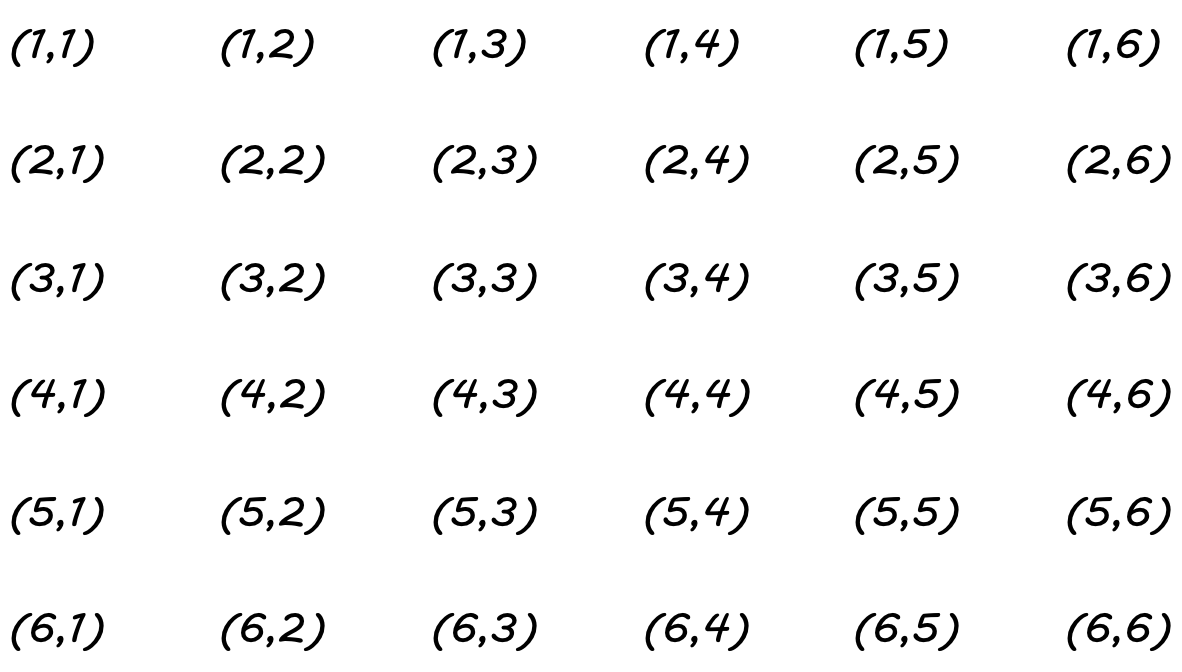
\includegraphics[scale=.32]{figs/SixesTable.png}

\end{frame}




\begin{frame}
\define{Conditional Probability}	
{
Let $E$,  and  $F$ are two events such that $P\left(\HLTY{F} \right)>0$, then the conditional probability of {\bf $\HLTEQ[amethyst!30]{E}$ given $\HLTY{F}$} is defined to be, 
\begin{center}
\qBrd[2.55in]{teal!30}{ $$ \vspace{-.01in}
\HLTW{\displaystyle P\left(\HLTEQ[amethyst!30]{E}\mid \HLTY{ F} \right):= \frac{P\left(\HLTEQ[amethyst!30]{E}\cap \HLTY{F}\right)}{P( \HLTY{F})}.} \vspace{-.01in}$$ }
\end{center}
}
\end{frame}



\begin{frame}{Example}
\vspace{-.3in}
\qbx[4.6in]{teal!30}{\Qn Suppose that a fair die is rolled once.  Find the conditional probability that $\HLTEQ[amethyst!30]{\text{\it  the number 1 appears}}$,  {\bf given } that \HLTY{\text{\it an odd number was obtained.}}
 }\\

\vspace{1.5in}
{\tiny 
A:= \{ Observe a 1.\}, 
B:=\{Observe an odd number.\}\\
 $P(A\mid B)=\frac{P(A\cap B)}{P(B)}=\frac{\frac{1}{6}}{\frac{3}{6}}=\frac{1}{3}.$}
\end{frame}






\begin{frame}{Example}
\vspace{-.1in}
\qbx[4.6 in]{teal!30}{\Qn \small  If two events, A and B, are such that $P( A)=0.5$, $P(B)=0.3$, and $P( A\cap B)= 0.1$, find the following
\begin{enumerate}
\item $P(A\mid B)$
\item $P(B\mid A)$
\item $P(A\mid A\cup B)$
\end{enumerate}
 }\\

\vspace{2.5in}

\end{frame}


%
%\begin{frame}\frametitle{Example}
%\qbx[4.5in]{apricot!70}{
%\Exmpl{apricot}{} A student is taking a one-hour-time-limit makeup examination.  Suppose the probability that the student will
%finish the exam in less than $x$ hours is $ \frac{x}{2}$, for all $0\leq x\leq 1.$ Then, given that the student is still working after $0.75$ hour, what is the conditional probability that the full hour is used?
%}\\
%%\pause
%\vspace{1in}
%{\tiny Solution: Let $L_x$ denote the event that the student finishes
%the exam in less than $x$ hours, $0\leq  x\leq 1$, and let $F$ be the
%event that the student uses the full hour.  Because $F$ is the
%event that the student is not finished in less than 1 hour, 
%$P(F)=P(\Not{L_1})=1-P(L_1)=0.5$.\\
%Now, the event that the student is still working at time $0.75$ is the complement of the event $L_{0.75}$, so the desired probability is obtained from
%$$P(F\mid \Not{L_{0.75}})= \frac{F\cap \Not{L_{0.75}}}{  \Not{L_{0.75}}  }= \frac{P(F)}{1- P(F_{0.75})}= \frac{0.5}{0.625}=0.8$$
%
%
%}
%\vspace{2in}
%
%\end{frame}





\begin{frame}\frametitle{Example}
\qbx[4.5in]{apricot!70}{
\Exmpl{apricot}{} A coin is flipped twice.  Assuming that all four
points in the sample space $\HLTW{\SampleS = \HLTY{ \{HH, HT, TH, TT\}}}$ are
equally likely, what is the conditional probability that both flips land on heads, given that (a) the first  flip lands on heads? 
(b) at least one flip lands on heads?
}\\
%\pause
%\vspace{1in}
{\tiny Solution: 

}
\vspace{2in}
\end{frame}





%
%
%\begin{frame}\frametitle{Example}
%\qbx[4.5in]{olive!40}{
%\Exmpl{olive}{} A total of $n$ balls are sequentially and randomly
%chosen, without replacement, from an urn containing $r$ red
%and b blue balls $(n \leq r + b)$. Given that $k$ of the $n$ balls are
%blue, what is the conditional probability that the first ball chosen is blue?
%}\\
%%\pause
%%\vspace{1in}
%{\tiny {\bf Solution:}   Show that this probability is $ \frac{k}{n}$.
%
%}
%\vspace{2in}
%\end{frame}
%
%
%





\begin{frame}
\define{Multiplication Rule of Probability }	
{
Let $E$ and $F$ are two events, then 
$$\HLTEQ[babyblue!70]{ \HLTY{P(E\cap F)}:=\HLTW{P(E\mid F)}\times \HLTW{P(F)}.}$$
}
\vspace{2.5in}
\end{frame}



%
%\begin{frame}\frametitle{Example}
%\qbx[4.5in]{teal!40}{
%\Exmpl{teal}{} Celine is undecided as to whether to take a
%French course or a chemistry course. She estimates that her
%probability of receiving an A grade would be $\frac{1}{2}$ in a French
%course and $\frac{2}{3}$ in a chemistry course. If Celine decides to
%base her decision on the  flip of a fair coin, what is the probability that she gets an A in chemistry?
%}\\
%%\pause
%%\vspace{1in}
%{\tiny {\bf Solution:}   .
%
%}
%\vspace{2in}
%
%\end{frame}


%
%
%\begin{frame}
%\define{ The Multiplication Rule:}	
%{
%$$P(E\cap F):=P(E\mid F)P(F).$$
%}
%\end{frame}


\begin{frame}\frametitle{Example}
\qbx[4.5in]{amber!40}{
\Exmpl{amber}{} Suppose that an urn contains 8 red balls and 4
white balls. We draw 2 balls from the urn without
replacement. If we assume that at each draw each ball in the
urn is equally likely to be chosen, what is the probability that
both balls drawn are red?
}\\
\pause
\vspace{1in}
{\tiny {\bf Solution:}  
Let $R_1$ and $R_2$ denote, respectively, the events that
the first and second balls drawn are red. Now, given that the
first ball selected is red, there are 7 remaining red balls and 4
white balls, so $P(R_2\mid R_1) =\frac{7}{11}$. . As $P(R_1) = \frac{8}{12}$ , the desired probability is
$$P(R_1\mid R_2) =P(R_2\mid R_1)\times P(R1)=\frac{7}{11}\frac{8
}{12}=\frac{14}{33}.$$

}
\vspace{2in}

\end{frame}








\begin{frame}


\qBrd[4.7in]{babyblue!70}{
$\HLTY{P(E_1\cap E_2\cap  E_3)} = \HLTW{P(E_1 \mid E_2\cap E_3 )} \times \HLTW{P(E_2\mid  E_3) } \times   \HLTW{P(E_{3})}.$
}

\qBrd[4.7in]{babyblue!70}{
\tiny  
$\HLTY{P(E_1\cap E_2\cap  E_3)}
{P(E_2\cap E_1\cap  E_3)}  = \HLTW{P(E_2 \mid E_1\cap E_3 )} \times \HLTW{P(E_1\mid  E_3) } \times   \HLTW{P(E_{3})}.$
}

\qBrd[4.75in]{babyblue!70}{
\tiny  
$\HLTY{P(E_1\cap E_2\cap  E_3)}
={P(E_3\cap E_2\cap  E_1)} = \HLTW{P(E_3 \mid E_2\cap E_1 )} \times \HLTW{P(E_2\mid  E_1) } \times   \HLTW{P(E_{1})}.$
}


\end{frame}


\begin{frame}

\qBrd[4.7in]{babyblue!70}{
$\HLTY{P(A\cap B\cap C)}
= \HLTW{P(A\mid B\cap C )} \times \HLTW{P(B\mid C) } \times   \HLTW{P(C)}.$
}

\qBrd[4.75in]{babyblue!70}{
\small $\HLTY{P(A\cap B\cap C \cap D)}
= \HLTW{P(A\mid B\cap C \cap D )} \times \HLTW{P(B\mid C\cap D ) } \times   \HLTW{P(C\mid D)}\times   \HLTW{P(D)}.$
}

\qBrd[4.75in]{babyblue!70}{
\tiny
 $\HLTY{P(A\cap B\cap C \cap D\cap E)}
= \HLTW{P(D\cap A\cap C \cap E \cap B )}=\HLTW{P(D\mid A\cap C \cap E \cap B )}  \times \HLTW{P( A\cap C \cap E \cap B  ) }.$
}

\end{frame}










\begin{frame}
\define{ The Generalized Multiplication Rule:}	
{
$P(E_1\cap E_2\cap \cdots E_k):=P(E_1) \times P(E_2\mid E_1)P(E_3\mid E_2\cap E_1 )\times \ldots \times P(E_k\mid E_1\cap E_2\cap \ldots\cap  E_{k-1}).$
}

\qBrd[4.7in]{babyblue!70}{
\vspace{-.15in}
\begin{eqnarray}
& & \HLTY{P(E_1\cap E_2\cap \cdots \cap E_k)} \nonumber\\
& :=& \HLTW{P(E_1 \mid E_2\cap \cdots \cap  E_k )} \times \HLTW{P(E_2\mid  E_3\cap  \cdots \cap E_k) } \times \ldots  \times\nonumber\\
& &\hspace{2.1in} \times  \HLTW{P(E_{k-1}\mid E_{k})}\times  \HLTW{P(E_{k})} .\nonumber
\end{eqnarray}
\vspace{-.15in}
}


\qBrd[4.7in]{unitednationsblue!60}{
\vspace{-.15in}
\begin{eqnarray}
& & \HLTY{P(E_1, E_2, \cdots , E_k)} \nonumber\\
& :=& \HLTW{P(E_1 \mid E_2, \cdots ,  E_k )} \times \HLTW{P(E_2\mid  E_3,  \cdots , E_k) } \times \ldots  \times\nonumber\\
& &\hspace{2.1in} \times  \HLTW{P(E_{k-1}\mid E_{k})}\times  \HLTW{P(E_{k})} .\nonumber
\end{eqnarray}
\vspace{-.15in}
}
\end{frame}



%
%\begin{frame}\frametitle{Example}
%\qbx[4.5in]{brightpink!40}{
%\Exmpl{brightpink}{} An ordinary deck of 52 playing cards is randomly
%divided into 4 piles of 13 cards each. Compute the probability
%that each pile has exactly 1 ace.
%}\\
%\pause
%\vspace{.9in}
%%{\tiny {\bf Solution:}  
%%Define events $E_i$, $i =1, 2, 3, 4$, as follows:
%%$E_1 = \{\text{the ace of spades is in any one of the piles}\},$\\
%%$E_2 = \{\text{the ace of spades and the ace of hearts are in different piles}\},$\\
%%$E_3 = \{\text{ the aces of spades, hearts, and diamonds are all in different piles}\},$\\
%%$E_4 = \{\text{all 4 aces are in different piles}\},$\\
%%
%%The desired probability is $P(E_1\cap E_2 \cap E_3 \cap E_4)$, and by the multiplication rule,
%%$P(E_1\cap E_2 \cap E_3 \cap E_4)=P(E_1) P( E_2\mid  E_1)P(E_3 \mid E_1 \cap E_2) P(   E_4 \mid E_1\cap E_2 \cap E_3 ) $\\
%%Note that 
%%$P(E_11) = 1$ ,  because $E_1$ is equal to the sample space.
%%$P(E_2\mid E_1) = \frac{39}{51}$, $P(E3\mid E_1 \cap  E_2) =-\frac{26}{50}$,  $P(E_4 \mid E_1\cap E_2 \cap E_3) = \frac{13}{49}.$\\ Therefore, 
%%$P(E_1\cap E_2 \cap E_3 \cap E_4)=P(E_1) P( E_2\mid  E_1)P(E_3 \mid E_1 \cap E_2) P(   E_4 \mid E_1\cap E_2 \cap E_3 =1 \times   \frac{39}{51}\times \frac{26}{50} \times  \frac{13}{49}  = 0.105$
%%}
%\vspace{2in}
%
%\end{frame}





\section{ Partition of an Event }
\TransitionFrame[amethyst]{\Large Partition of an Event Using Partion of Sample Space}

{
%\setbeamercolor{structure}{fg=antiquefuchsia!80, bg= black!60}
\setbeamercolor{structure}{fg=gray!30, bg= black!60}


\begin{frame}
	\frametitle{Reminder from Unit1 Slides: Disjoint Sets}
	\vspace{-.1in}
	\begin{center}
\qbx[4.3in]{teal!30}{\qBrd[1in]{olive!30}{\bf Disjoint Sets:}  Two sets  A, and  B are said to be  {\bf Disjoint Sets} or {\bf mutually exclusive sets} if $A$ and $B$ does not have any elements in common.\\
}\\
\vspace{-.2in}
  \qbx[3in]{applegreen!50}{  
 A and B are Disjoint $\Leftrightarrow \HLTY{A\cap B=\emptyset}$.
  }
  
  	\end{center}
	\vspace{4in}
	\end{frame}
	



\begin{frame}
	\frametitle{Reminder from Unit1 Slides: Partition}
	\vspace{-.1in}
	\begin{center}
\qbx[4.6in]{antiquebrass!60}{\qBrd[.8in]{olive!30}{\bf Partition:}  A collection of sets $\HLTY{\{A_1, A_2, \cdots, A_k\}}$ is called a {\bf partition for a set $\HLTW{C}$} if
\begin{enumerate}
\item  \qBrd[3.5in]{applegreen!30}{$A_i \cap A_j = \emptyset$ for $1\leq i \neq j \leq k$ ({\tiny  i.e. ,$A_i$,  and $A_j$ are Disjoint if $i\neq j$}) }, and 
\item  \qBrd[4in]{teal!30}{$\HLTY{A_1\cup A_2\cup \cdots \cup  A_k} =\HLTW{C}$.}
\end{enumerate}
}\\
%\pause
\vspace{.1in}
  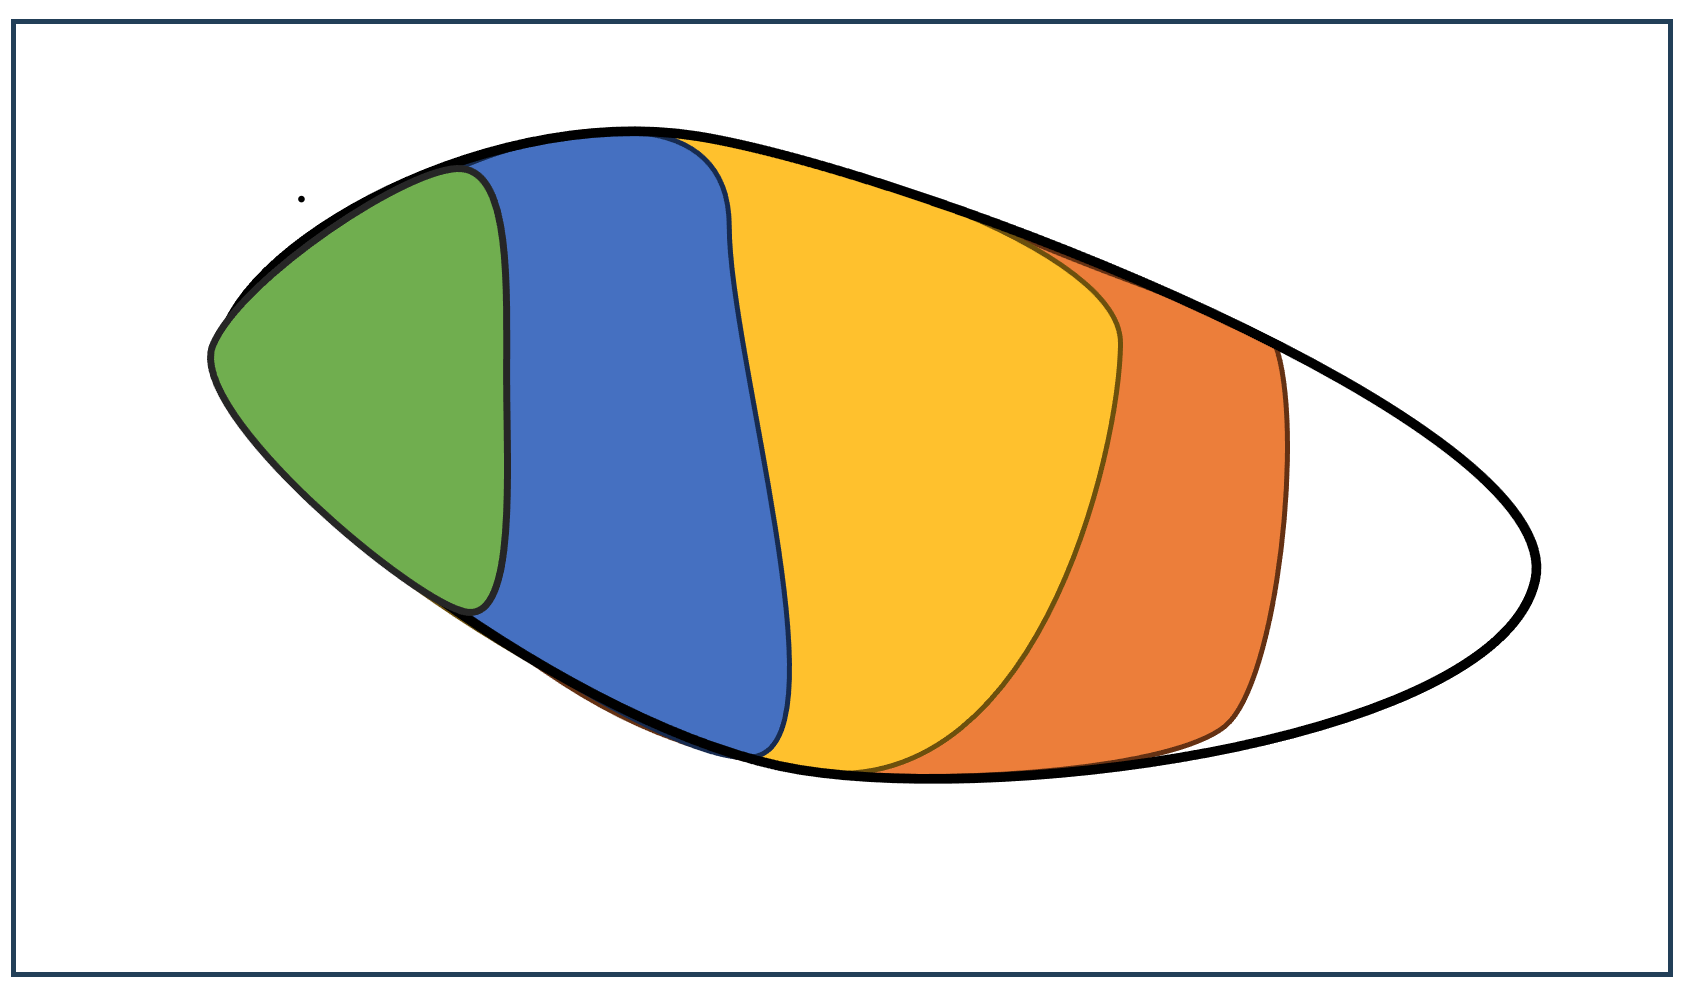
\includegraphics[scale=.22]{figs/VDPartition2.png} 
  	\end{center}
  	
	\vspace{4in}
	\end{frame}


}





\begin{frame}\frametitle{  Partition of Sample Space}
\vspace{-.2in}
	\begin{center}
\qbx[4.6in]{amethyst!60}{\qBrd[1.9in]{olive!30}{\bf Partition of Sample Space:}  A collection of sets $\HLTY{\{A_1, A_2, \cdots, A_n\}}$ is called a {\bf partition } for a set $\HLTW{\SampleS}$ if
\begin{enumerate}
  \item\qBrd[3.7in]{applegreen!30}{  the collection of events  $\HLTY{\{A_i\}_{i=1}^{n}}$ are {\bf pairwise disjoint} }
 , and 
 \item \qBrd[2.5in]{teal!30}{ $\HLTY{A_1\cup A_2\cup \cdots \cup  A_n} =\HLTW{\SampleS}$.}
\end{enumerate}
}\\
%\pause
%\vspace{.1in}
 % 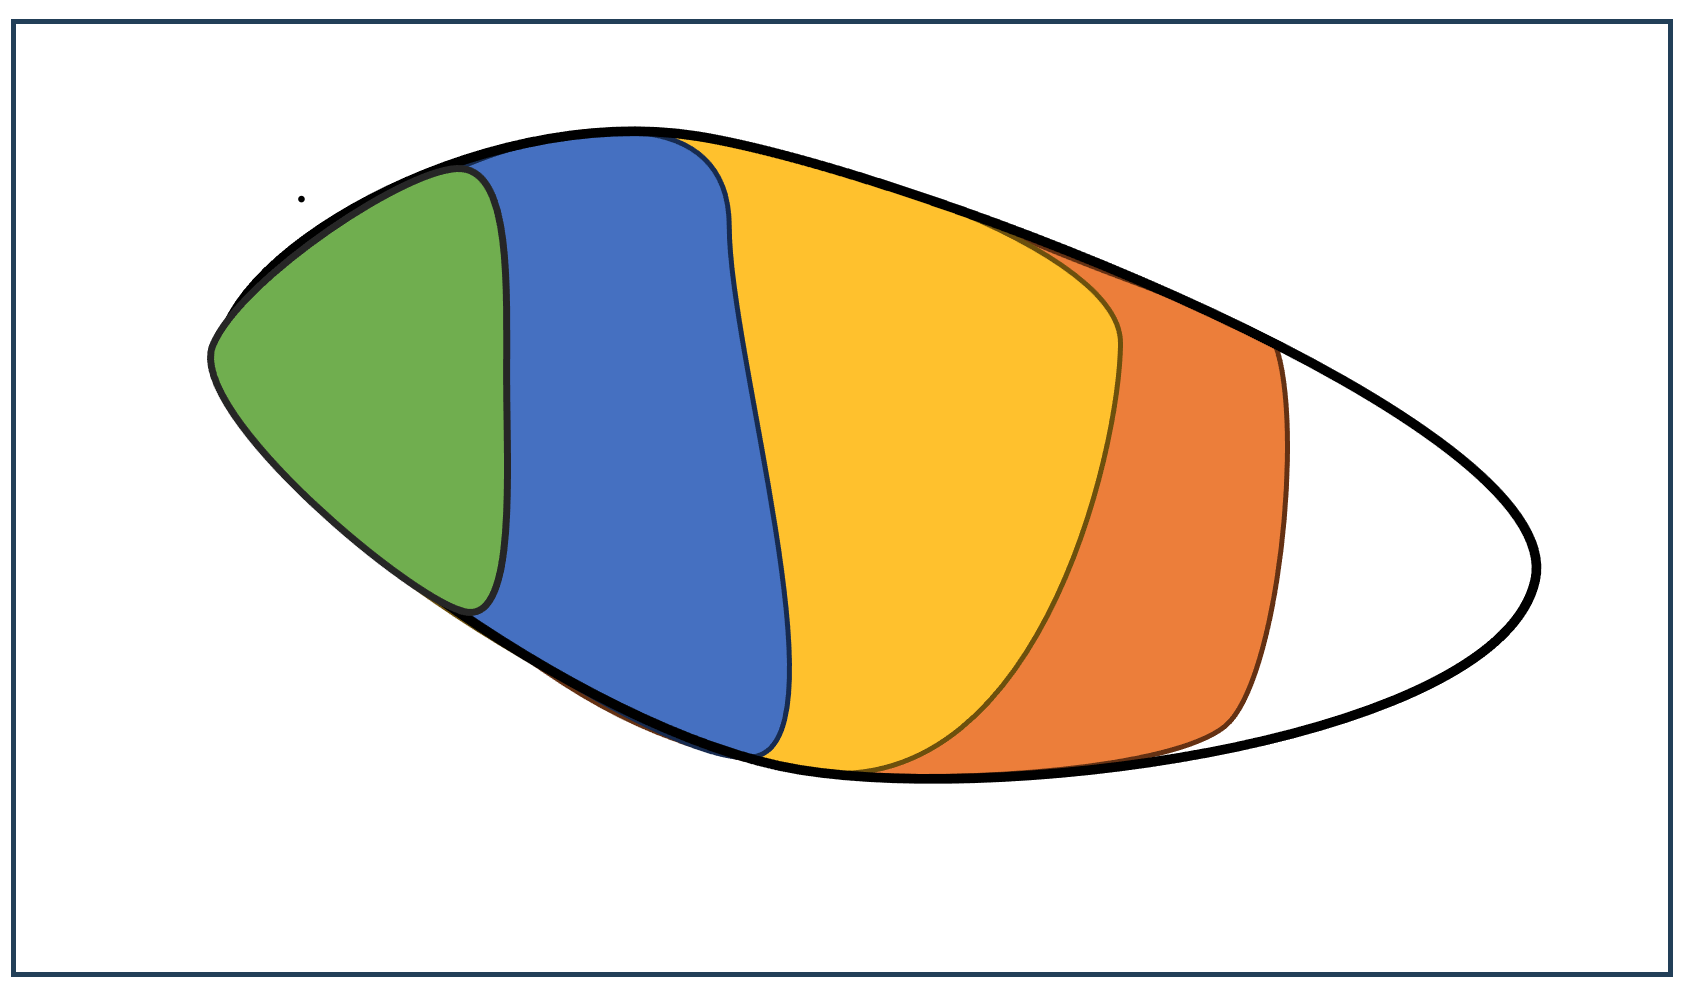
\includegraphics[scale=.2]{figs/VDPartition2.png} 
  	\end{center}
  	



\vspace{.1in}

\qBrd[4.5in]{bittersweet!50}{\HLTW{
Comment:}In the above definition, we may replace $\HLTY{n}$ by $\HLTY{\infty}$ and the definition extends naturally. }
\pause
\vspace{.1in}

\qBrd[4.5in]{teal!50}{\HLTW{
Comment:} Any set $\HLTY{A}$ and  it's complement,  $\HLTY{\Not{A}}$,  creates  a partition of $\HLTW{\SampleS}$.}


\end{frame}






\begin{frame}
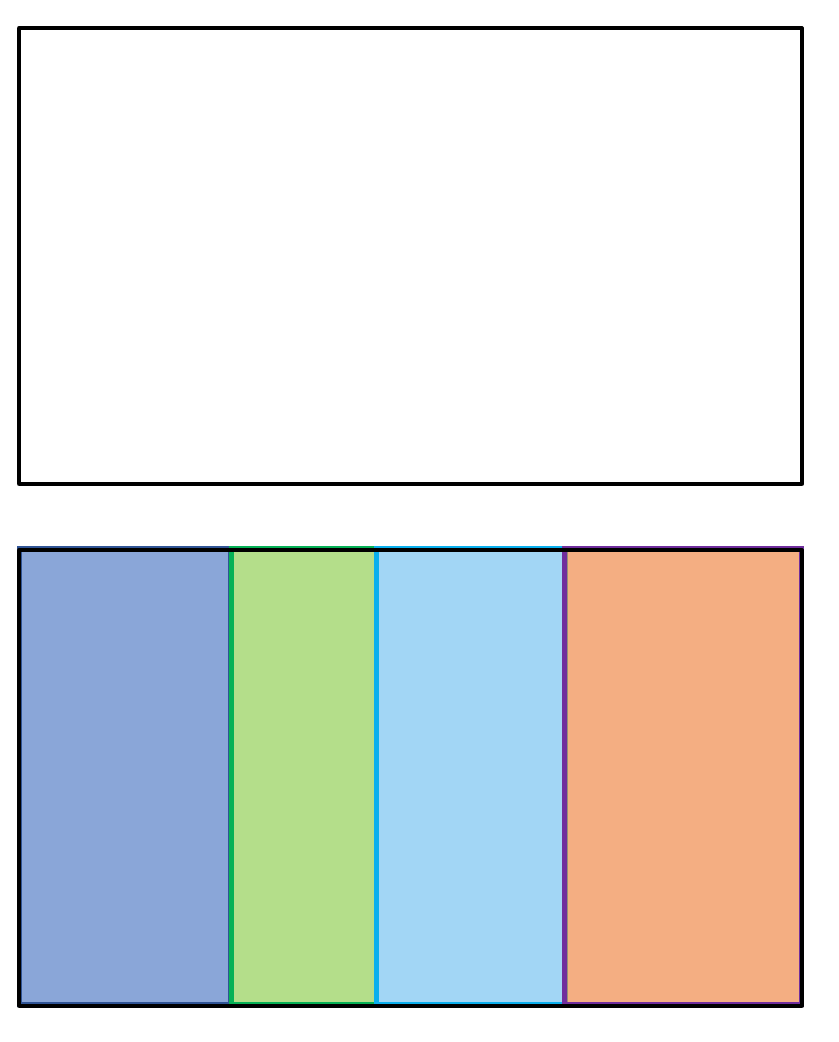
\includegraphics[scale=.4]{figs/PartitionUnivSet.png}
\end{frame}
\begin{frame}
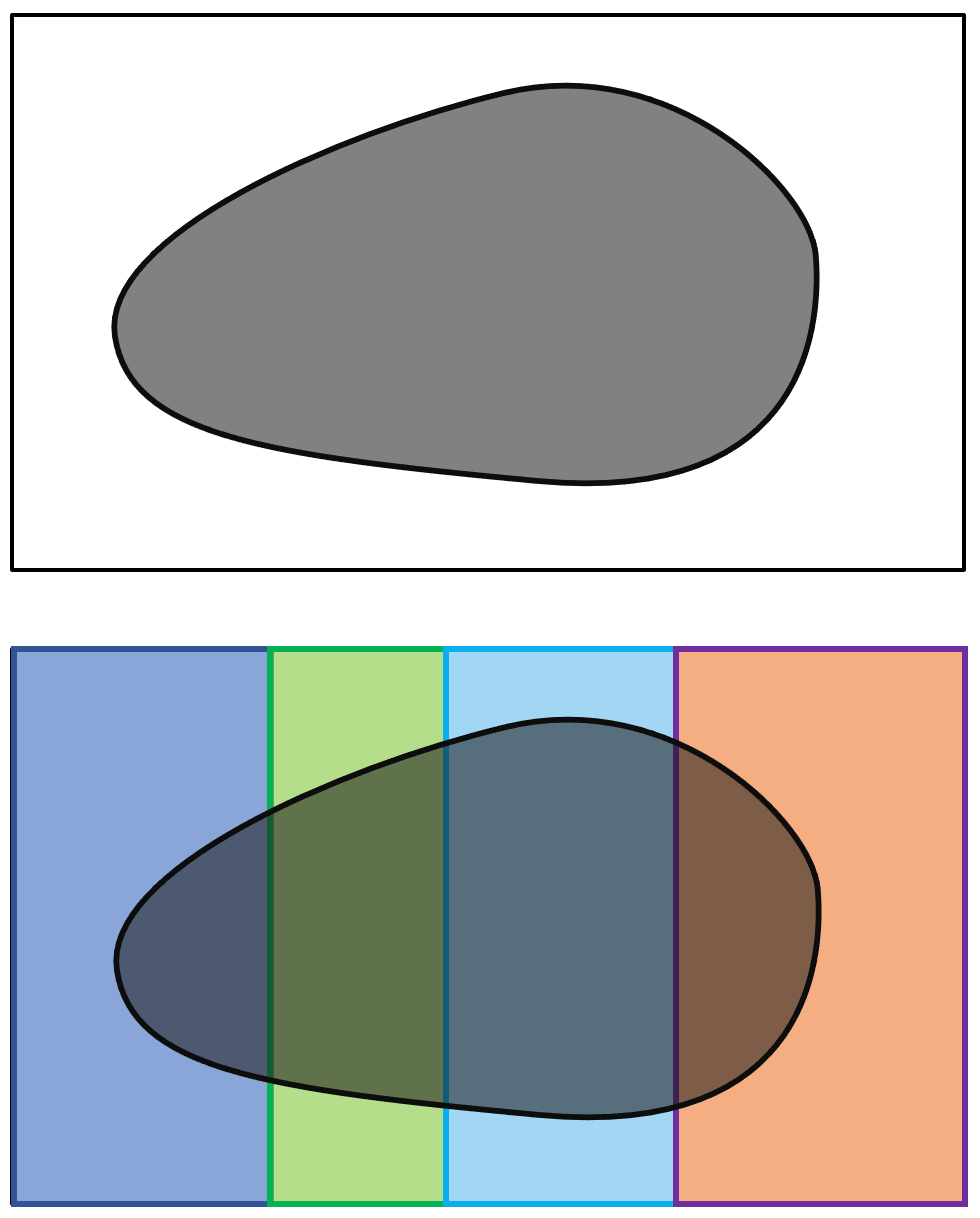
\includegraphics[scale=.4]{figs/PartitionOfE.png}
\end{frame}


\begin{frame}
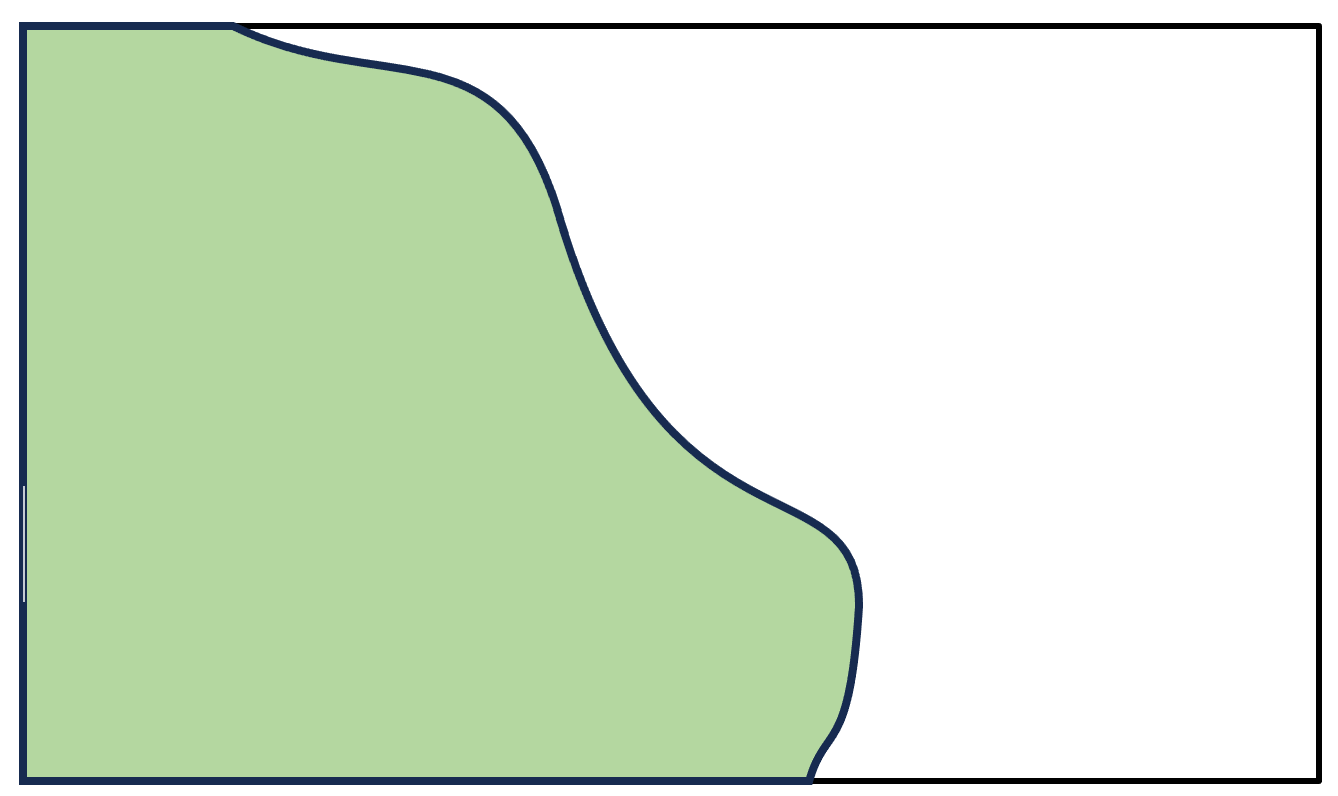
\includegraphics[scale=.25]{figs/TwoSetPartionS.png}\pause
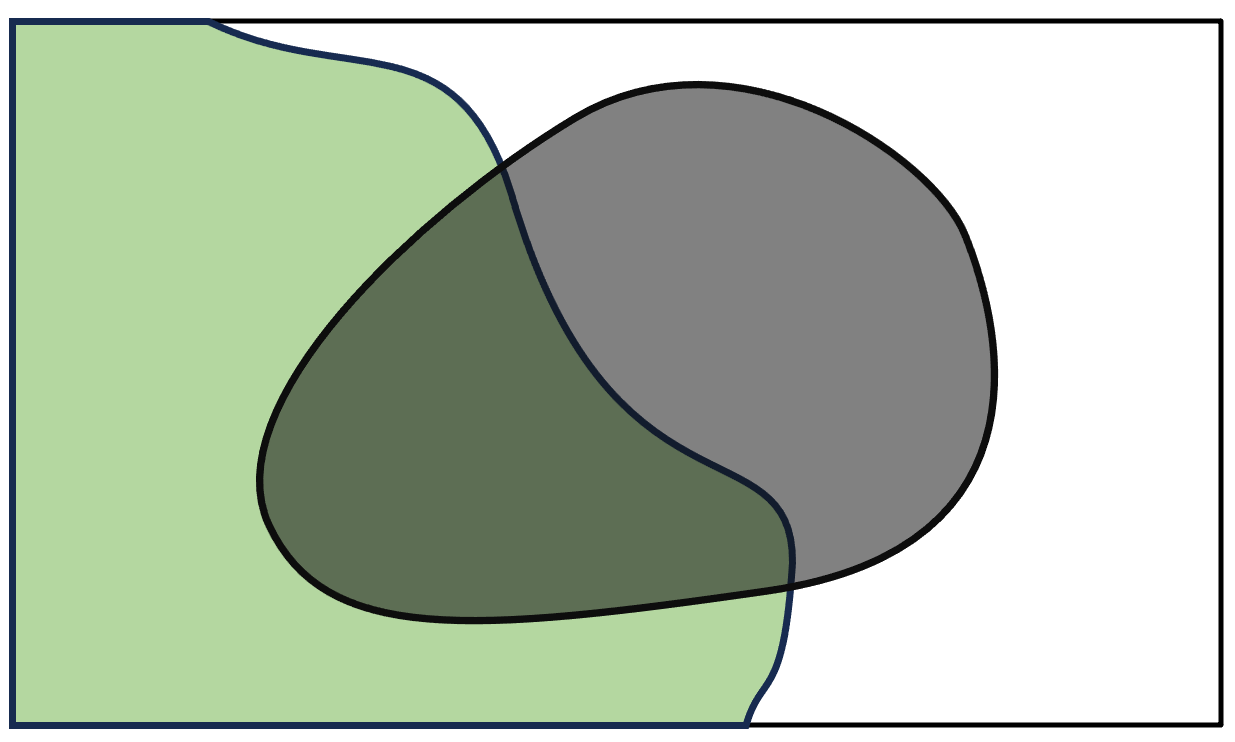
\includegraphics[scale=.27]{figs/Law_of_Total_Probability_Simple.png}
\vspace{1.5in}
\end{frame}



\section{Law of Total Probability}
\TransitionFrame[amethyst]{\Large Law of Total Probability}


\begin{frame}\frametitle{Law of  Total Probability}
\begin{center}
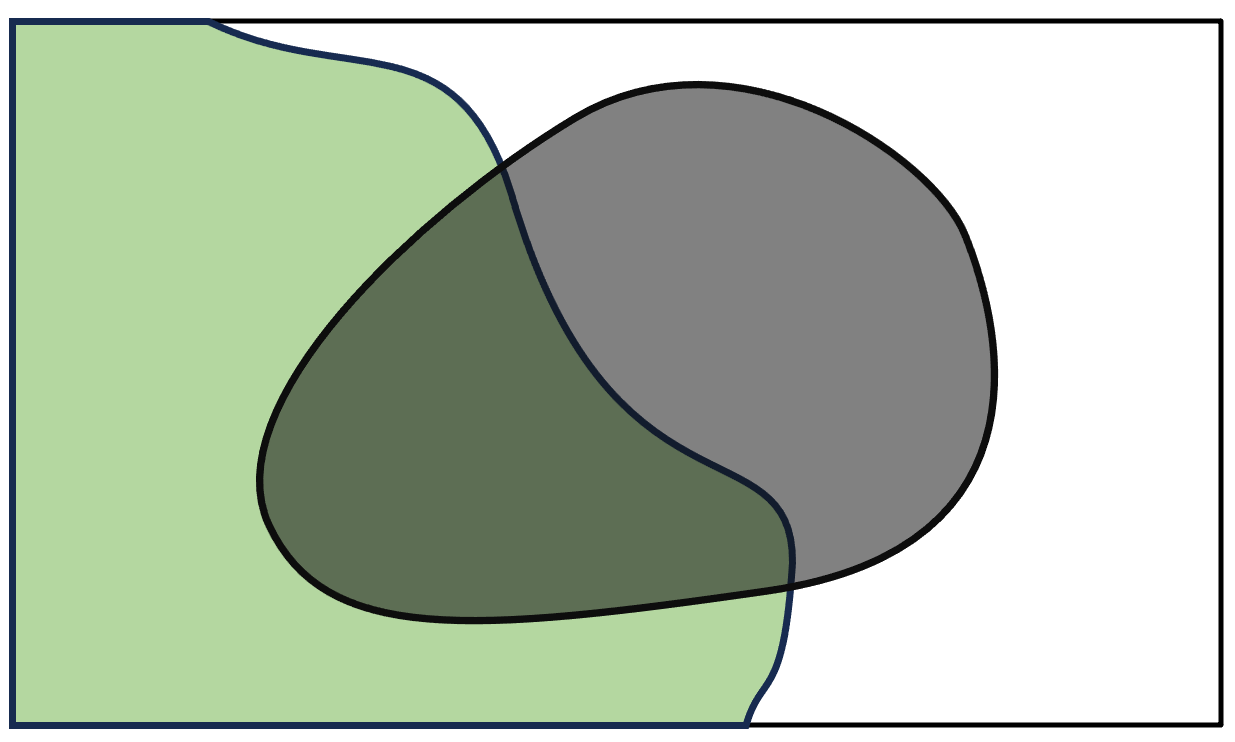
\includegraphics[scale=.35]{figs/Law_of_Total_Probability_Simple.png} 
\vspace{.2in}\\
\qBrd[2in]{babyblue!70}{$ \HLTEQ[gray!20]{E}= \HLTEQ[applegreen!70]{(E\cap F)} \cup \HLTW{(E\cap \Not{F})} $}\\
\vspace{.08in}
\qBrd[2.6in]{unitednationsblue!40}{$ \HLTEQ[gray!20]{P(E)}= \HLTEQ[applegreen!70]{P(E\cap F) }+ \HLTW{P(E\cap \Not{F})} $  }
\end{center}
\vspace{.5in}
\end{frame}



\begin{frame}\frametitle{Law of  Total Probability}
\qbx[4.5in]{teal!40}{
Let E and F be two events, then 
\begin{center}
\qBrd[3in]{babyblue!90}{$ \HLTEQ[gray!20]{ P(E)} = \HLTY{\HLTEQ[applegreen!70]{P(E\mid F)P(F) } +  \HLTW{P(E\mid  \Not{F}))(\Not{F})}} $}
\end{center}
\vspace{.2in}
}

\vspace{1.5in}
\end{frame}

\begin{frame}\frametitle{Law of  Total Probability (General)}
\begin{center}
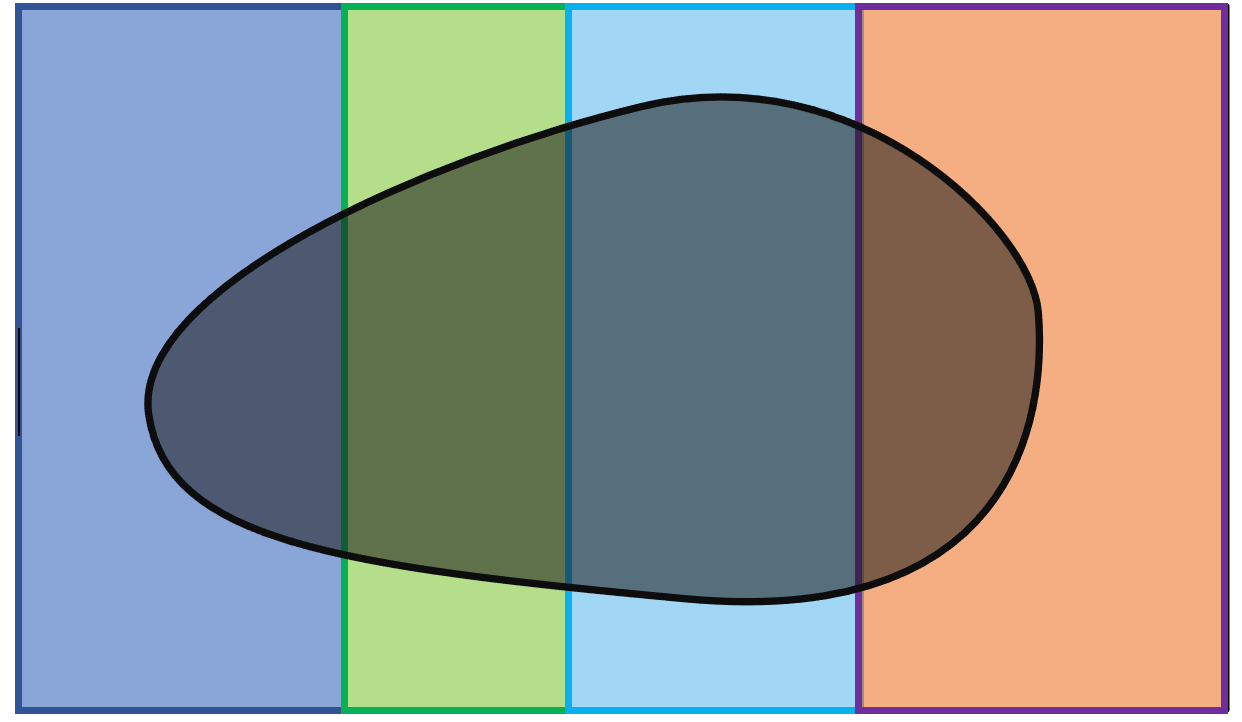
\includegraphics[scale=.35]{figs/Law_of_Total_Probability.png} 
\end{center}
\vspace{.4in}
\end{frame}

\begin{frame}\frametitle{Law of  Total Probability (General)}
\vspace{-.1in}

\qbx[4.5in]{turquoisegreen!90}{
\qBrd[2.4in]{yellow-green!50}{Law of  Total Probability (General):} Let E be an event.  Assuming that the collection of sets   $\{F_1, F_2,\ldots,  F_k\}$  forms a partition of $\SampleS$,  we have
\vspace{-.15in}
\begin{center}
%\qBrd[2in]{applegreen!40}{$ E= (E\cap F) \cup (E\cap \Not{F}) $}\\
\qBrd[3in]{green!40}{$\displaystyle P(E)=\HLTW{\sum_{j=1}^{k}  P(E\mid F_j)P(F_j)  }$}
\end{center}
}

\vspace{1.5in}

\end{frame}






\begin{frame}\frametitle{Example}
\vspace{-.1in}
\qbx[4.5in]{applegreen!40}{
\Exmpl{applegreen}{} An insurance company believes that people can be divided into two classes: those who are accident prone and those who are not. 
The companys statistics show that an accident-prone person will have an accident at some time within a fixed 1-year period with probability $0.4$, whereas this probability is $0.2$ for a person who is not accident prone.  If we assume that $30\%$
 of the population is accident prone, what is the probability
that a new policyholder will have an accident within a year of
purchasing a policy?
}\\
\pause
\vspace{.6in}
{\tiny {\bf Solution:}  
 Let $A_1$ denote the event that the policyholder will have an accident within a year of purchasing
the policy, and let $A$ denote the event that the policyholder is accident prone. Hence, the desired probability is given by
$P(A_1) = P(A_1\mid A)P(A) + P(A1\mid \Not{A})P(\Not{A}) = (0.4)(0.3)+(0.2)(0.7	)=0.26$
}
\end{frame}










\section{Bayes' Theorem}
\TransitionFrame[amethyst]{\Large Bayes' Theorem  }


\begin{frame}

\begin{theorem}
Let $\HLTW{F_1, F_2, \ldots,  F_{_K}}$ be a set of mutually exclusive and exhaustive events (meaning that exactly one of these events must occur).  Suppose now that $E$ has occurred and we are interested in determining which one of the $F_j$ also occurred. Then, we have the following theorem\\
\ \vspace{-.2in}
$$\DBX{ \displaystyle P(F_i \mid E)=\HLTW{ \frac{ \displaystyle P(E\mid F_i) P(F_i )}{\displaystyle \sum_{j=1}^{K}P(E\mid F_j) P(F_j) }}}$$
\end{theorem}



\end{frame}


\begin{frame}
\begin{itemize}
\item This theorem is well known as Bayes's theorem, after the
English philosopher {\bf Thomas Bayes}.
\vspace{.25in}


\item We can use the following Applet to find the conditional
probability using Bayes's theorem:
\vspace{.25in}




\item \url{http://www.thomsonedu.com/statistics/book_
content/0495110817_wackerly/applets/seeingstats/
Chpt2/bayesTree.html}
\end{itemize}



\end{frame}






\begin{frame}\frametitle{Example}
\vspace{-.1in}
\qbx[4.5in]{amethyst!40}{
\Exmpl{amethyst}{}  An insurance company believes that people can be divided into two classes: those who are accident prone and those who are not. 
The companys statistics show that an accident-prone person will have an accident at some time within a fixed 1-year period with probability $0.4$, whereas this probability is $0.2$ for a person who is not accident prone.  If we assume that $30\%$
 of the population is accident prone. \\
 Suppose that a new policyholder has an accident within a year of purchasing a policy. What is the probability that he or she is accident prone?
}\\
\pause
\vspace{.6in}
{\tiny {\bf Solution:}  
 The desired probability is 
 $$P(A\mid A_1)=  \frac{P(A\cap A_1)}{P(A_1)}= \frac{(0.4)(0.3)}{0.26}= \frac{6}{13} $$
}
\end{frame}



%__________________________________________
\begin{frame}{ Bayes' Theorem: Example   }
\vspace{-.1in}
\qBox{\Qn:
A diagnostic test for a disease is such that it (correctly) detects the disease in 90\% of the
individuals who actually have the disease. Also, if a person does not have the disease, the test
will report that he or she does not have it with probability 0.9. Only 1\%  of the population has the
disease in question. If a person is chosen at random from the population and the diagnostic test
indicates that she has the disease, what is the conditional probability that she does, in fact, have
the disease? Are you surprised by the answer? Would you call this diagnostic test reliable?}

\pause 
\vspace{.1in}

{\tiny 
$A=\{ \text{The individial has the disease} \},  \Not{A}=\{ \text{ does not have the disease} \}$, 
$ B=\{ \text{The test shows a POSITIVE result}\}$
$\Not{B}=\{ \text{The test shows a NEGATIVE result}\}$

$\HLTEQ[yellow]{ P(B\mid A)=0.9, P(\Not{B}\mid A^c)=0.9 \text{ and  } P(A)=0.01}$
 $$P(A\mid B)= \frac{P(B\mid A)P(A)}{  P(B\mid A)P(A)+ P(B\mid \Not{A})P(\Not{A}) }= \frac{(0.9)(0.01)}{(0.9)(0.01)+ (0.1)(0.99)}=91\%$$
}

\end{frame}


\begin{frame}\frametitle{Example}
\vspace{-.1in}
\qbx[4.5in]{atomictangerine!40}{
\Exmpl{atomictangerine}{}     Suppose that we have 3 cards that are identical in form, except that both sides of the first card are colored red, both sides of the second card are colored black, and one side of the third card is colored red and the other side black. The 3 cards are mixed up in a hat, and 1 card is randomly selected and put down on the ground. If the upper side of the chosen card is colored red, what is the probability that the other side is colored black?
}\\
\pause
\vspace{.6in}
{\tiny {\bf Solution: Let RR, BB, and RB denote, respectively, the events that the chosen card is all red, all black, or the redblack card. Also, let R be the event that the upturned side of the chosen card is red. Then
the desired probability is obtained
$$    P(RB\mid R)=  \frac{P(R\mid RB)P(RB)}{P(R\mid RR)P(RR)+ P(R\mid RB)P(RB) + P(R\mid BB)P(BB)}= \frac{\frac{1}{2}\times \frac{1}{3} }{   (1)\times \frac{1}{3}  + \frac{1}{2}\times \frac{1}{3}  +  (0) \times  \frac{1}{3}      }=  \frac{1}{3}   .$$   
}  

}
\end{frame}






\begin{frame}\frametitle{Example}
\vspace{-.1in}
\qbx[4.5in]{olive!40}{
\Exmpl{olive}{}     A new couple, known to have two children, has just moved into town. Suppose that the mother is encountered walking with one of her children. If this child is a girl, what is the probability that both children are girls?
}\\
\pause

{\tiny {\bf Solution:   

}  
\vspace{1.6in}
}
\end{frame}





\begin{frame}\frametitle{Example}
\vspace{-.1in}
\qbx[4.5in]{teal!40}{
\Exmpl{teal!40}{}    
The length, width, and height of a manufactured part are classified as being either within or outside specified tolerance limits. In a quality inspection $86\%$ of the parts are found to be within the specified tolerance limits for width, but only $80\%$ of the parts are within the specified tolerance limits for all three dimensions. However,  $2\%$ of the parts are within the specified tolerance limits for width and length but not for height, and $3\%$ of the parts are within the specified tolerance limits for width and height but not for length. Moreover, $92\%$ of the parts are within the specified tolerance limits for either width or height, or both of these dimensions.
\begin{enumerate}
\item If a part is within the specified tolerance limits for height, what is the probability that it will also be within the specified tolerance limits for width?
\item If a part is within the specified tolerance limits for length and width, what is the probability that it will be within the specified tolerance limits for all three dimensions?
\end{enumerate}
}\\
%\pause

{\tiny {\bf Solution:   

}  
\vspace{1.6in}
}
\end{frame}






\begin{frame}\frametitle{Example}
\vspace{-.1in}
\qbx[4.5in]{babyblue!40}{
\Exmpl{babyblue!40}{}    
A car repair is either on time or late and either
satisfactory or unsatisfactory. If a repair is made on time,
then there is a probability of 0.85 that it is satisfactory. There is a probability of 0.77 that a repair will be made on time. What is the probability that a repair is made on time and is satisfactory?
\begin{enumerate}
\item
\item 
\end{enumerate}
}\\
%\pause

{\tiny {\bf Solution:   

}  
\vspace{1.6in}
}
\end{frame}







\begin{frame}\frametitle{Example}
\vspace{-.1in}
\qbx[4.5in]{olive!40}{
\Exmpl{olive!40}{}    
An island has three species of bird. Species 1 accounts for
$45\%$ of the birds, of which $10\%$ have been tagged. Species
$2$ accounts for $38\%$ of the birds, of which $15\%$ have been tagged. Species 3 accounts for $17\%$ of the birds, of which
$50\%$ have been tagged. If a tagged bird is observed, what
are the probabilities that it is of species 1, of species 2, and
of species 3?
}\\
%\pause

{\tiny {\bf Solution:   

}  
\vspace{1.6in}
}
\end{frame}




\begin{frame}\frametitle{Example}
\vspace{-.1in}
\qbx[4.5in]{olive!40}{
\Exmpl{olive!40}{}    
An island has three species of bird. Species 1 accounts for
$45\%$ of the birds, of which $10\%$ have been tagged. Species
$2$ accounts for $38\%$ of the birds, of which $15\%$ have been tagged. Species 3 accounts for $17\%$ of the birds, of which
$50\%$ have been tagged. If a tagged bird is observed, what
are the probabilities that it is of species 1, of species 2, and
of species 3?
}\\
%\pause

{\tiny {\bf Solution:   

}  
\vspace{1.6in}
}
\end{frame}








\begin{frame}\frametitle{Example}
\vspace{-.1in}
\qbx[4.5in]{airforceblue!40}{
\Exmpl{airforceblue!40}{}    
After production, an electrical circuit is given a quality
score of A, B, C, or D. Over a certain period of time,
$77\%$ of the circuits were given a quality score A,
$11\%$ were given a quality score B, $7\%$ were given a
quality score C, and $5\%$ were given a quality score D.
Furthermore, it was found that $2\%$ of the circuits given a
quality score A eventually failed, and the failure rate was
$10\%$ for circuits given a quality score B, $14\%$ for circuits
given a quality score C, and $25\%$ for circuits given a
quality score D.
}\\
%\pause

{\tiny {\bf Solution:   

}  
\vspace{1.6in}
}
\end{frame}






\begin{frame}\frametitle{Example}
\vspace{-.1in}
\qbx[4.5in]{airforceblue!40}{
\Exmpl{airforceblue!40}{}    
After production, an electrical circuit is given a quality
score of A, B, C, or D. Over a certain period of time,
$77\%$ of the circuits were given a quality score A,
$11\%$ were given a quality score B, $7\%$ were given a
quality score C, and $5\%$ were given a quality score D.
Furthermore, it was found that $2\%$ of the circuits given a
quality score A eventually failed, and the failure rate was
$10\%$ for circuits given a quality score B, $14\%$ for circuits
given a quality score C, and $25\%$ for circuits given a
quality score D.
}\\
%\pause

{\tiny {\bf Solution:   

}  
\vspace{1.6in}
}
\end{frame}




\begin{frame}\frametitle{Example}
\vspace{-.1in}
\qbx[4.5in]{amethyst!50}{
\Exmpl{amethyst!45}{}    
The length, width, and height of a manufactured part are classified as being either within or outside specified tolerance limits. In a quality inspection $86\%$ of the parts are found to be within the specified tolerance limits for width, but only $80\%$ of the parts are within the specified tolerance limits for all three dimensions. However,  $2\%$ of the parts are within the specified tolerance limits for width and length but not for height, and $3\%$ of the parts are within the specified tolerance limits for width and
}\\
\pause

{\tiny {\bf Solution:   

}  
\vspace{1.6in}
}
\end{frame}





%
%\begin{frame}\frametitle{Example}
%\vspace{-.1in}
%\qbx[4.5in]{teal!40}{
%\Exmpl{teal}{}     A bin contains 3 different types of disposable
%ashlights. The probability that a type 1 
%ashlight will give over 100 hours of use is .7, with the corresponding probabilities for type 2 and type 3  ashlights being .4 and .3, respectively. Suppose that 20 percent of the  ashlights in the bin are type 1, 30 percent are type 2, and 50 percent are type 3.
%}\\
%\pause
%
%{\tiny {\bf Solution:   
%
%}  
%\vspace{1.6in}
%}
%\end{frame}
%





\begin{frame}\frametitle{Example}
\vspace{-.1in}
\qbx[4.5in]{teal!40}{
\Exmpl{teal}{}     A bin contains 3 different types of disposable
ashlights. The probability that a type 1 
ashlight will give over 100 hours of use is 0.7, with the corresponding probabilities for type 2 and type 3  ashlights being 0.4 and 0.3, respectively. Suppose that 20 percent of the  ashlights in the bin are type 1,  30 percent are type 2, and 50 percent are type 3.
\begin{enumerate}
\item What is the probability that a randomly chosen 
ashlight will give more than 100 hours of use?
\item Given that a  ashlight lasted over 100 hours, what is the conditional probability that it was a type j  ashlight, j = 1, 2, 3?
\end{enumerate}
}\\
%\pause

{\tiny {\bf Solution:   

}  
\vspace{1.6in}
}
\end{frame}




\begin{frame}\frametitle{Example}
\vspace{-.1in}
\qbx[4.5in]{antiquefuchsia!40}{
\Exmpl{antiquefuchsia}{}     We know the following about a colormetric method used to test lake water for nitrates. If
water specimens contain nitrates, a solution dropped into the water will cause the specimen to
turn red 95\% of the time. When used on water specimens without nitrates, the solution causes
the water to turn red 10\% of the time (because chemicals other than nitrates are sometimes
present and they also react to the agent). Past experience in a lab indicates that nitrates are
contained in 30\%of the water specimens that are sent to the lab for testing. If a water specimen is randomly selected
\begin{enumerate}
\item from among those sent to the lab, what is the probability that it will turn red when tested?
\item It it turns red when tested, what is the probability that it actually contains nitrates?
\end{enumerate}
}\\
%\pause

{\tiny {\bf Solution:   

}  
\vspace{1.6in}
}
\end{frame}




\begin{frame}\frametitle{Example}
\vspace{-.1in}
\qbx[4.5in]{olive!40}{
\Exmpl{olive}{}     When a organisation's website is accessed, there is a probability of 0.07 that the web address
was typed in directly. In such a case, there is a probability of 0.08 that an online purchase
will be made. On the other hand, when the website is accessed indirectly, which occurs with
probability 0.93, then there is only a 0.01 chance that an online purchase will be made. 
\begin{enumerate}
\item The probability that the website is accessed directly and that a purchase is made ? %0.0056
\item What is the probability that the website is accessed indirectly and that a purchase is made? %0.0093
\item  What proportion of online purchases are from individuals who access the website directly?%0.376
\end{enumerate}
}\\
%\pause

{\tiny {\bf Solution:   

}  
\vspace{1.6in}
}
\end{frame}



\section{The Notion of Statistical Independence }
\TransitionFrame[amethyst]{\Large The Notion of Statistical Independence }




\begin{frame}\frametitle{Statistical Independence }
\define{Statistically Independent Event}{
Two events $E$ and $F$ are said to be  statistically independent if
$$\DBX{\displaystyle P(E\cap F ) = P(E)\times P(F)    }$$
}



\pause 

\begin{center}
\qBrd[4.1in]{amethyst!60}{Corollary: Two events E and F are independent if and only
if $P(E\mid F) = P(E)$ and $P(F\mid E) = P(F).$
}
\end{center}
\end{frame}


\begin{frame}\frametitle{Example}
\vspace{-.1in}
\qbx[4.5in]{amber!40}{
\Exmpl{amber}{}    A card is selected at random from an ordinary deck of 52 playing cards. If E is the event that the selected card is an ace and F is the event that it is a spade, then E and F are independent.
}\\
\pause

{\tiny {\bf Solution:   
This follows because $P(E\cap F) = \frac{1}{52}$ whereas
$P(E) = \frac{4}{52}$ and $P(F) = \frac{13}{52}.$
}  
\vspace{1.6in}
}
\end{frame}



\begin{frame}\frametitle{Example}
\vspace{-.1in}
\qbx[4.5in]{amber!40}{
\Exmpl{amber}{}   Two coins are 
flipped, and all 4 outcomes are assumed to be equally likely.  If E is the event that the first coin lands on heads and F the event that the second lands on tails, then E and F are independent, since
$P(E \cap F)= P(\{HT\})= \frac{1}{4}$. Where as $P(E)= P(\{HH, HT\})=\frac{1}{2}$ and $P(F)= P(\{HT, TT\})=\frac{1}{2}$ 
}\\
%\pause

%{\tiny {\bf Solution:   
%This follows because $P(E\cap F) = \frac{1}{52}$ whereas
%$P(E) = \frac{4}{52}$ and $P(F) = \frac{13}{52}.$
%}  
\vspace{1.6in}
%}
\end{frame}




\begin{frame}\frametitle{Example}
\vspace{-.1in}
\qbx[4.5in]{babyblue!40}{
\Exmpl{babyblue}{}   Suppose that we toss 2 fair dice. Let $E_1$ denote the
event that the sum of the dice is 6 and F denote the event that the
first die equals 4.  Is $E_1$ statistically independent of $F$?\\
}\\
%\vspace{.1in}
%\qbx[4.5in]{asparagus!40}{
%\Exmpl{asparagus}{}   Now, suppose that we let $E_2$ be the event that the sum of the dice equals $7$.   Is $E_2$ statistically independent of $F$?\\
%\HLTW{\text{Answer:} }
%$P(E_2\cap F)= P(\{(4,3)\})= \frac{1}{36}$ where as $P(E_2)=\frac{1}{6}$ and $P(F)= \frac{1}{6}$.  Therefore,  $E_2$ and $F$ are  statistically independet because, 
%$P(E_2 \cap F)= P(E_2) \times P( F) $.
%}\\
%\pause

%{\tiny {\bf Solution:   
%This follows because $P(E\cap F) = \frac{1}{52}$ whereas
%$P(E) = \frac{4}{52}$ and $P(F) = \frac{13}{52}.$
%}  
%\vspace{1.6in}
%}
\vspace{1.5in}
{\tiny \HLTW{\text{Answer:} }
   $P(E_1 \cap F)= P(\{(4,2)\})= \frac{1}{36}$ where as $P(E_1)=\frac{5}{36}$ and $P(F)= \frac{1}{6}$.  Therefore,  $E_1$ and $F$ are not statistically independet because, 
$P(E_1 \cap F)\neq P(E_1) \times P( F) $.}
\end{frame}





\begin{frame}\frametitle{Example}
\vspace{-.1in}
%\qbx[4.5in]{babyblue!40}{
%\Exmpl{babyblue}{}   Suppose that we toss 2 fair dice. Let $E_1$ denote the
%event that the sum of the dice is 6 and F denote the event that the
%first die equals 4.  Is $E_1$ statistically independent of $F$?\\
%\HLTW{\text{Answer:} }
%   $P(E_1 \cap F)= P(\{(4,2)\})= \frac{1}{36}$ where as $P(E_1)=\frac{5}{36}$ and $P(F)= \frac{1}{6}$.  Therefore,  $E_1$ and $F$ are not statistically independet because, 
%$P(E_1 \cap F)\neq P(E_1) \times P( F) $.
%}\\
%\vspace{.1in}
\qbx[4.5in]{asparagus!40}{
\Exmpl{asparagus}{}   Now, suppose that we let $E_2$ be the event that the sum of the dice equals $7$.   Is $E_2$ statistically independent of $F$?
}\\
\vspace{1.7in}
%\pause

%{\tiny {\bf Solution:   
%This follows because $P(E\cap F) = \frac{1}{52}$ whereas
%$P(E) = \frac{4}{52}$ and $P(F) = \frac{13}{52}.$
%}  
%\vspace{1.6in}
%}
{\tiny \HLTW{\text{Answer:} }
$P(E_2\cap F)= P(\{(4,3)\})= \frac{1}{36}$ where as $P(E_2)=\frac{1}{6}$ and $P(F)= \frac{1}{6}$.  Therefore,  $E_2$ and $F$ are  statistically independet because, 
$P(E_2 \cap F)= P(E_2) \times P( F) $.}
\end{frame}






\begin{frame}
\qBrd[4.5in]{teal!40}{ \HLTW{Proposition:} If two events $A$, and $B$ are statistically independent, then 
\begin{enumerate}[a).]
\item  $A$ and $\Not{B}$ are also statistically independent, 
\item  $\Not{A}$ and ${B}$ are also statistically independent. 
\item  $\Not{A}$ and $\Not{B}$ are also statistically independent. 
\end{enumerate}
}
{\tiny Solution:}
\vspace{2in}
\end{frame}






\begin{frame}\frametitle{Example}
\vspace{-.1in}
\qbx[4.5in]{teal!40}{
\Exmpl{teal}{}   If A and B are independent events with P( A) = 0.5 and P( B) = 0.2, find the following:
\begin{enumerate}
\item $P(A\cap B)$
\item $P(A\cup B)$
\item $P(\Not{A}\cap \Not{B})$
\item $P(\Not{A}\cup \Not{B})$
\end{enumerate}
}\\
\pause

{\tiny {\bf Solution:   

}  
\vspace{1.6in}
}
\end{frame}



\begin{frame}\frametitle{Example}
\vspace{-.1in}
\qbx[4.5in]{teal!40}{
\Exmpl{teal}{}  Three radar sets, operating independently, are set to detect any aircraft flying through a certain area. Each set has a probability of $.02$ of failing to detect a plane in its area. If an aircraft enters the area, what is the probability that it
\begin{enumerate}
\item goes undetected?
\item is detected by at least one  radar set?
\item is detected by all three radar sets?
\end{enumerate}
}\\
\pause

{\tiny {\bf Solution:   

}  
\vspace{1.6in}
}
\end{frame}





\begin{frame}\frametitle{Example}
\vspace{-.1in}
\qbx[4.5in]{amber!40}{
\Exmpl{amber}{}    A card is selected at random from an ordinary deck of 52 playing cards. If E is the event that the selected card is an ace and F is the event that it is a spade, then E and F are independent.
}\\
\pause

{\tiny {\bf Solution:   
This follows because $P(E\cap F) = \frac{1}{52}$ whereas
$P(E) = \frac{4}{52}$ and $P(F) = \frac{13}{52}.$
}  
\vspace{1.6in}
}
\end{frame}

 

\begin{frame}\frametitle{Relation between:  Statistical  Independence \& Disjointness   }
\vspace{-.1in}
\qbx[4.5in]{amethyst!40}{
{\HLTW{Result}:   If $A$ and $B$ are two  events such that $P(A)>0$ and $P(B>0)$ then, 
\begin{enumerate}[a).]
\item If the events A and B are Statistically Independent then they can not be disjoint./mutually exclushive. 
\item If the events A and B are disjoint then they can not be statistically independent. 
\end{enumerate}
   }  
}\\

\vspace{1.5in}
\end{frame} 
 
 

\begin{frame}\frametitle{Generalized Definition of Statistical Independence }
\define{Statistically Independent Events}{
Three events $A_1$, $A_2$, and $A_3$ are said to be  statistically independent if
\begin{center}
\qBrd[3.5in]{applegreen!40}{ $P(A_1\cap A_1 \cap A_3 ) = P(A_1)\times P(A_2)  \times P(A_3)  $}\\
\qBrd[2.5in]{purple!30}{ $P(A_1\cap A_2 ) = P(A_1)\times P(A_2)  $}\
\qBrd[2.5in]{amethyst!30}{ $P(A_1\cap A_3 ) = P(A_1)\times P(A_3)  $}\\
\qBrd[2.5in]{bittersweet!40}{ $P(A_2\cap A_3 ) = P(A_2)\times P(A_3)  $}\\

\end{center}
}
\vspace{1.5in}

\end{frame}



\begin{frame}\frametitle{Example}
\vspace{-.1in}
\qbx[4.5in]{almond!40}{
\Exmpl{almond}{}   A biased  coin is tossed 3 tiimes. Assume that the tosses are independent to each other (Means events concerning only toss 1 is statistically independent to events concerning toss 2).  Assume that the probability for Head for the toss is $\pi$ ($\pi$ is any number between 0 to 1, for example $\pi=0.75$).  Therefore all the outcomes in the sample space may not be equally likelly.  Find the probability of the following events
\begin{enumerate}
\item  $\{HHH\}$
\item  $\{HHT\}$,  $\{THH\}$, $\{HTH\}$
\item  Exactly one of the toss results in a Head. 
\item  Exactly two of the tosses result in Head. 
\end{enumerate}
}\\
%\pause

%{\tiny {\bf Solution:   
%This follows because $P(E\cap F) = \frac{1}{52}$ whereas
%$P(E) = \frac{4}{52}$ and $P(F) = \frac{13}{52}.$
%}  
\vspace{1.6in}
%}
\end{frame}



\TransitionFrame[antiquefuchsia]{\Large Questions?  }
 
 
 
\end{document}
